%Metodología
\section{Metodología}\label{sec:metodologia}
    \subsection{Parte 1. Osciladores}

    \begin{figure}[H]
      \centering
      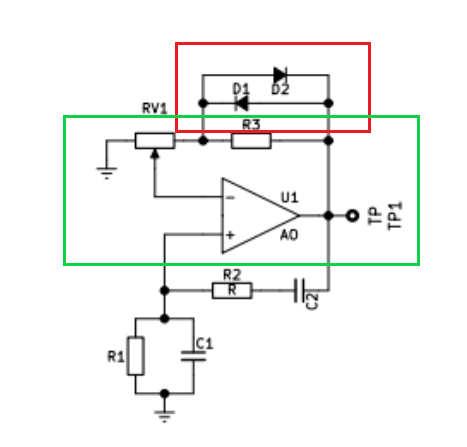
\includegraphics[width=8cm]{Circuitos/puente_wien_control.png}
      \caption{Oscilador de Puente de Wien con control de amplitud. Cuadro Rojo: Control de amplitud. Cuadro Verde: Aplica Método de Amplificador Desvanecido}
      \label{fig:puente_wien_control}
    \end{figure}

        
    \begin{enumerate}
    
        \subsubsection{Diseño} 
        
        \item Para el circuito de la figura \ref{fig:puente_wien_control}, determine la frecuencia de oscilación.
            \textbf{Nota:} Los siguientes cálculos se realizan sin el control de amplitud para hallar los datos de diseño.
            
            Observando la figura \ref{fig:puente_wien_control}, aplicamos el Método de Amplificador Desvanecido, desarrollando se obtiene lo siguiente, tomando en cuenta el estudio de un oscilador donde su ciclo de ganancia es $\beta A = 1$.

            \begin{gather}
                \text{Recordando que $A=X_{31}$ y $\beta = A_f$ para efectiva aplicar MAD,}\nonumber\\[0.5cm]
                A_f=1+\left(\dfrac{R_3+XR_{v1}}{R_{v1}(1-X)}\right) \label{eqn:af} 
            \end{gather}

            para simplificar los cálculos y el diseño $R_1=R_2=R$ y $C_1=C_2=C$, por lo tanto, se tiene:
            
            \begin{gather}
                X_{31}=\dfrac{e_1}{e_3}=\dfrac{R||\dfrac{1}{SC}}{R||\dfrac{1}{SC}+R+\dfrac{1}{SC}}=\dfrac{\dfrac{\dfrac{R}{SC}}{R+\dfrac{1}{SC}}}{\dfrac{\dfrac{R}{SC}}{R+\dfrac{1}{SC}}+R+\dfrac{1}{SC}}\nonumber \\[0.5cm]
                X_{31}=\dfrac{\dfrac{R}{RSC+1}}{\dfrac{R}{RSC+1}+\dfrac{RSC+1}{SC}}=\dfrac{\dfrac{R}{RSC+1}}{\dfrac{RSC+(RSC+1)^2}{SC(RSC+1)}}\nonumber \\[0.5cm]
                X_{31}=\dfrac{RSC}{RSC+(RSC)^2+2RSC+1}=\dfrac{RSC \, A_f}{S^2(RC)^2+S(3RC)+1}  \nonumber \\[0.5cm]
                A_fX_{31}=\dfrac{RSC \, A_f}{S^2(RC)^2+S(3RC)+1} \label{eqn:afx31}
            \end{gather}

            Con la ecuación \ref{eqn:afx31}, se aplicará el criterio de Barkhausen.

            \begin{align}
                \begin{cases}
                    RSC(A_f)=3RC \\[0.5cm]
                    S^2(RC)^2+1=0 
                \end{cases}
                \label{eqn:1}
            \end{align}

            Despejando $S$ de la segunda ecuación del sistema de ecuaciones \ref{eqn:1} y conociendo que $S=\sigma + jw=jw $, sustituyendo queda:

            \begin{gather}
                S^2=-\dfrac{1}{(RC)^2}=(jw)^2=-w^2 \Longrightarrow w=\sqrt{\dfrac{1}{(RC)^2}}=\dfrac{1}{(RC)^2} \nonumber  \\[0.5cm]
                \text{La frecuencia que oscila es, }\nonumber  \\[0.5cm]
                w=\dfrac{1}{(RC)^2} \label{eqn:w}
            \end{gather}

            Ahora hallamos la Ganancia, con la primera ecuación del sistema de ecuaciones  \ref{eqn:1}, se tiene:

            \begin{gather}
                RCSA_f=3RCS \Rightarrow A_f=3=1+\dfrac{R_3+XR_{v1}}{R_{v1}(1-X)} \label{eqn:af2}
            \end{gather}

        \item Diseñe (especifique valores comerciales, para cada elemento) el oscilador de la Figura \ref{fig:puente_wien_control} para obtener una frecuencia de oscilación de 5.0 KHz.

            La frecuencia de oscilación de la figura \ref{fig:puente_wien_control}, es la siguiente:

            Haciendo uso de la ecuación \ref{eqn:af2}, se obtiene $R$,

            \begin{gather}
                w=\dfrac{1}{(RC)^2}=2\pi f \Longrightarrow R= \dfrac{1}{C2\pi f} \label{eqn:R}
            \end{gather}

            Asumiendo $C=10 \, nF$, tenemos,

            \begin{gather}
                R=\dfrac{1}{(10n)(2\pi)(5k)}=3.183 \, k\ohm \approx 3.3 \, k \ohm \nonumber  \\[0.5cm]
                \text{Siendo un valor comercial,} R=3.3 \, k \ohm
            \end{gather}

        \item Determine la amplitud de la señal de salida cuando está presente el control de amplitud.

            Se tomara en cuenta $X=0.4$, se sabe que en la ecuación \ref{eqn:af2} tenemos:

            \begin{gather}
                3 = 1 + \frac{R_3 + XR_{v1}}{R_{v1}(1-X)} \Longrightarrow \frac{R_3 + 0.4R_{v1}}{R_{v1}(1-0.4)} \nonumber \\[0.5cm]
                R_3 + 0.4R_{v1} = 2(0.6R_{v1}) = 1.2R_{v1} \nonumber \\[0.5cm]
                R_3 = 1.2R_{v1} - 0.4R_{v1} = 0.8R_{v1} \nonumber \\[0.5cm]
                \text{Asumiendo que } R_{v1} = 10k\ohm \quad \therefore \quad R_3 = 0.8(10k) = 8 \, k\ohm \approx 8.2 \, \ohm \nonumber
            \end{gather}

            Estos valores estabilizan su oscilación si variamos el potenciómetro, este puede tener 2 estados más que puede ser en corto o saturación.

            Para hallar esos estados se tomara en cuenta lo siguiente:

            \begin{gather}
                \dfrac{R_3+XR_{v1}}{R_{v1}(1-X)}>2 \nonumber \\[0.5cm]
                R_3+XR_{v1}>2R_{v1}-2XR_{v1} \quad \Rightarrow \quad R_{v1}(x+2x-2)>-R_3 \nonumber \\[0.5cm]
                3x>-\dfrac{R_3}{R_{v1}}+2 \quad \Rightarrow \quad x>\dfrac{1}{3}\left(-\dfrac{R_3}{R_{v1}}+2 \right) \nonumber
            \end{gather}

            Sabiendo que $R_3=8.2 \, k \ohm$ y $R_{v1}=10 \, k \ohm$ se tiene,

            $x>0.39 \approx 0.4$

            Ahora tomando en cuenta lo siguiente, desarrollamos,

            \begin{gather*}
                \dfrac{XR_{v1}}{R_{v1}(1-X)}<2 \quad \Rightarrow  \quad x<2-2X \\[0.5cm]
                3X<2 \quad \Rightarrow  \quad x<\dfrac{2}{3} \approx 0.67
            \end{gather*}

            Obteniendo el siguiente intervalo, $$0.4<X<0.67$$ 

            Que es donde el circuito va a oscilar en los valores del potenciómetro.
        
        \subsubsection{Simulación}
        
        \item Realice la simulación de la etapa con el fin de verificar el modelo teórico y las condiciones de oscilación obtenidas a partir de el. Verifíquese además la amplitud de salida con y sin control de amplitud.

            \begin{itemize}
                \item \textbf{Sin Control de Amplitud}

                      \begin{figure}[H]
                        \centering
                        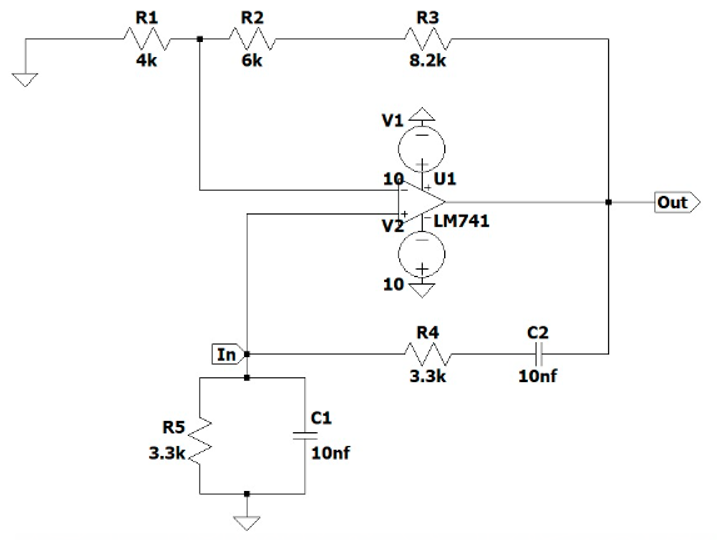
\includegraphics[width=8cm]{Imagenes/sim_cir_puente_wien_sc6.png}
                        \caption{Circuito sin control de amplitud de la Figura \ref{fig:puente_wien_control} cuando X=0.40.}
                        \label{fig:sim_cir_puente_wien_sc6}
                    \end{figure}

                    \begin{figure}[H]
                        \centering
                        \renewcommand{\figurename}{Gráfica}
                        \setcounter{figure}{0}
                        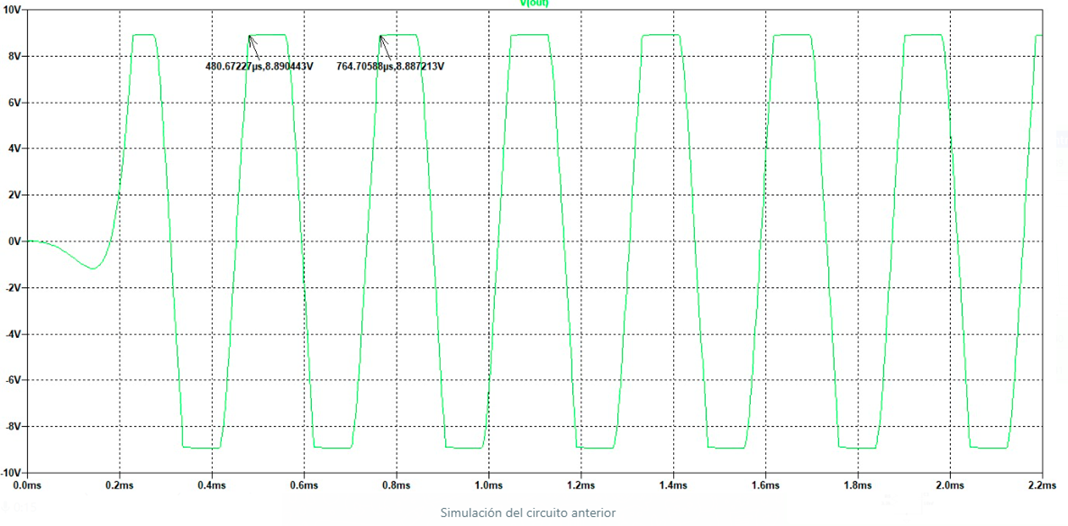
\includegraphics[width=15cm]{Imagenes/sim_puente_wien_sc6.png}
                        \caption{Simulación sin control de amplitud de la Figura \ref{fig:puente_wien_control} cuando X=0.40. Saturado}
                        \label{fig:sim_puente_wien_sc6}
                    \end{figure}

                      \begin{figure}[H]
                        \centering
                        \setcounter{figure}{5}
                        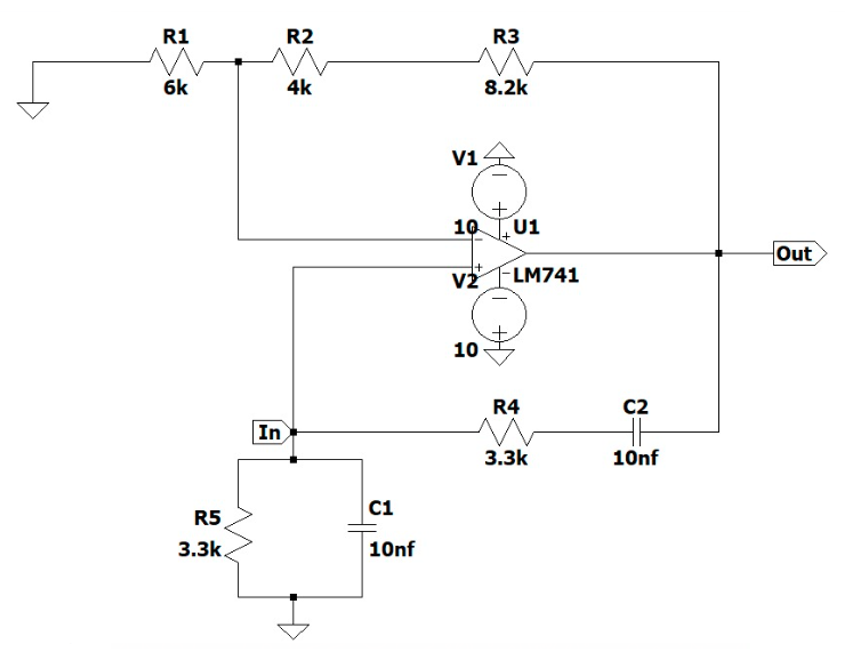
\includegraphics[width=8cm]{Imagenes/sim_cir_puente_wien_sc4.png}
                        \caption{Circuito sin control de amplitud de la Figura \ref{fig:puente_wien_control} cuando X=0.60.}
                        \label{fig:sim_cir_puente_wien_sc4}
                    \end{figure}

                    \begin{figure}[H]
                        \centering
                        \renewcommand{\figurename}{Gráfica}
                        \setcounter{figure}{1}
                        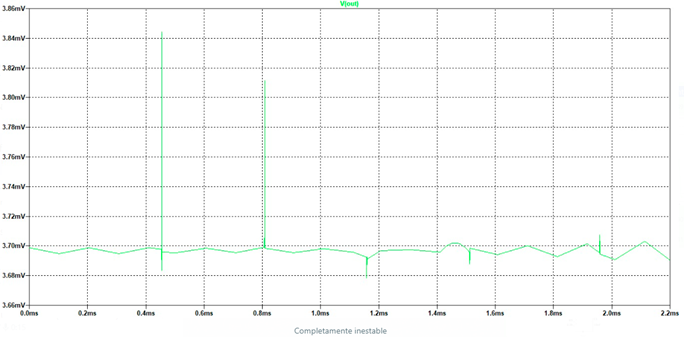
\includegraphics[width=15cm]{Imagenes/sim_puente_wien_sc4.png}
                        \caption{Simulación sin control de amplitud de la Figura \ref{fig:puente_wien_control} cuando X=0.60. Inestable}
                        \label{fig:sim_puente_wien_sc4}
                    \end{figure}

                    \begin{figure}[H]
                        \centering
                        \setcounter{figure}{6}
                        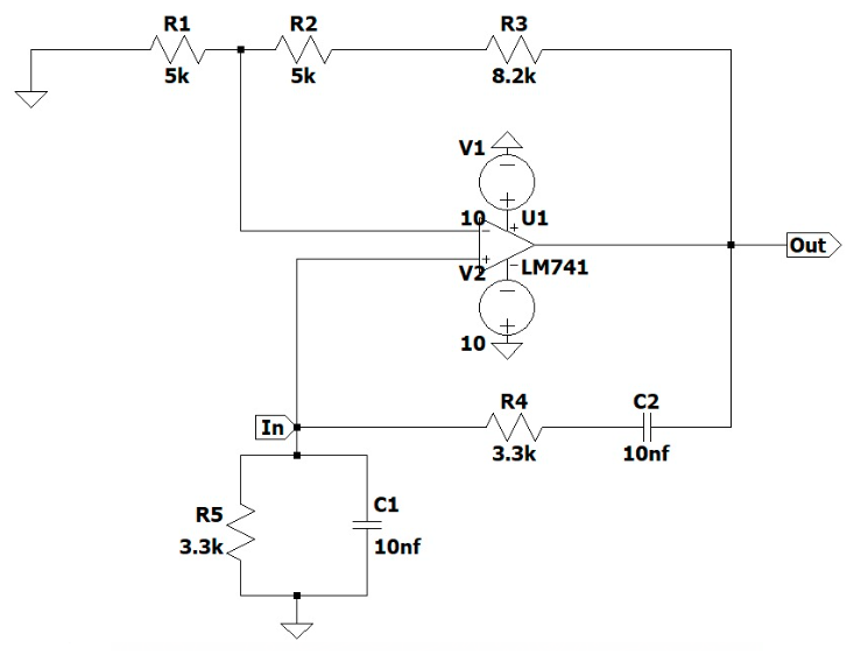
\includegraphics[width=8cm]{Imagenes/sim_cir_puente_wien_sc5.png}
                        \caption{Circuito sin control de amplitud de la Figura \ref{fig:puente_wien_control} cuando X=0.5.}
                        \label{fig:sim_cir_puente_wien_sc5}
                    \end{figure}

                    \begin{figure}[H]
                        \centering
                        \renewcommand{\figurename}{Gráfica}
                        \setcounter{figure}{2}
                        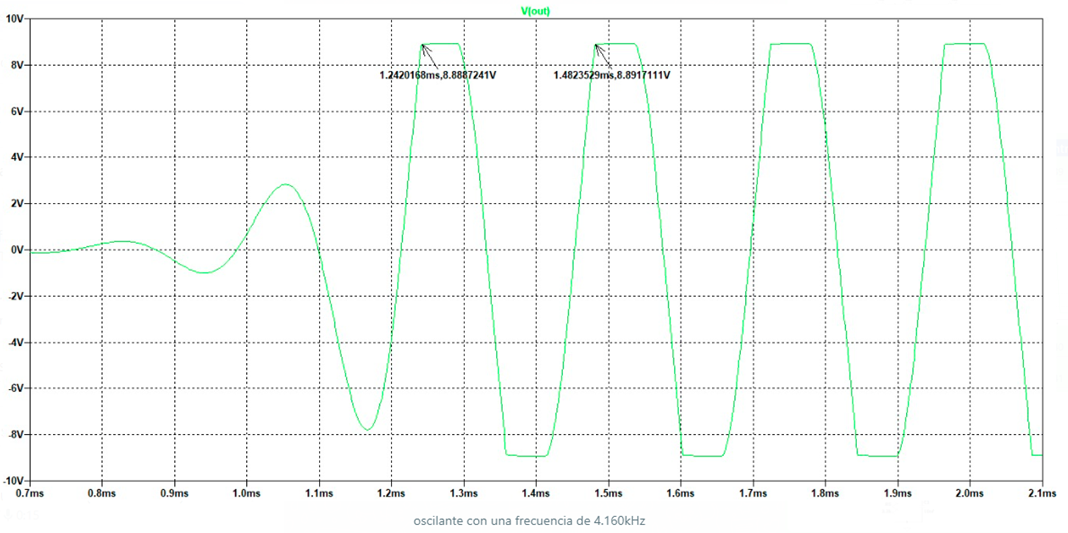
\includegraphics[width=15cm]{Imagenes/sim_puente_wien_sc5.png}
                        \caption{Simulación sin control de amplitud de la Figura \ref{fig:puente_wien_control} cuando X=0.5. Saturado}
                        \label{fig:sim_puente_wien_sc5}
                    \end{figure}

                    \begin{figure}[H]
                        \centering
                        \setcounter{figure}{7}
                        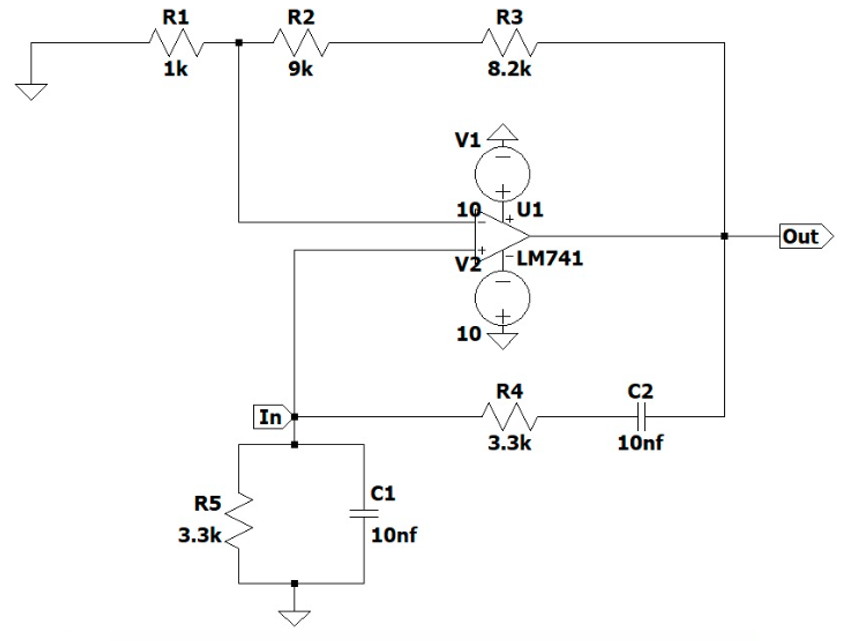
\includegraphics[width=8cm]
                        {Imagenes/sim_cir_puente_wien_sc9.png}
                        \caption{Circuito sin control de amplitud de la Figura \ref{fig:puente_wien_control} cuando X=0.10.}
                        \label{fig:sim_cir_puente_wien_sc9}
                    \end{figure}

                    \begin{figure}[H]
                        \centering
                        \renewcommand{\figurename}{Gráfica}
                        \setcounter{figure}{3}
                        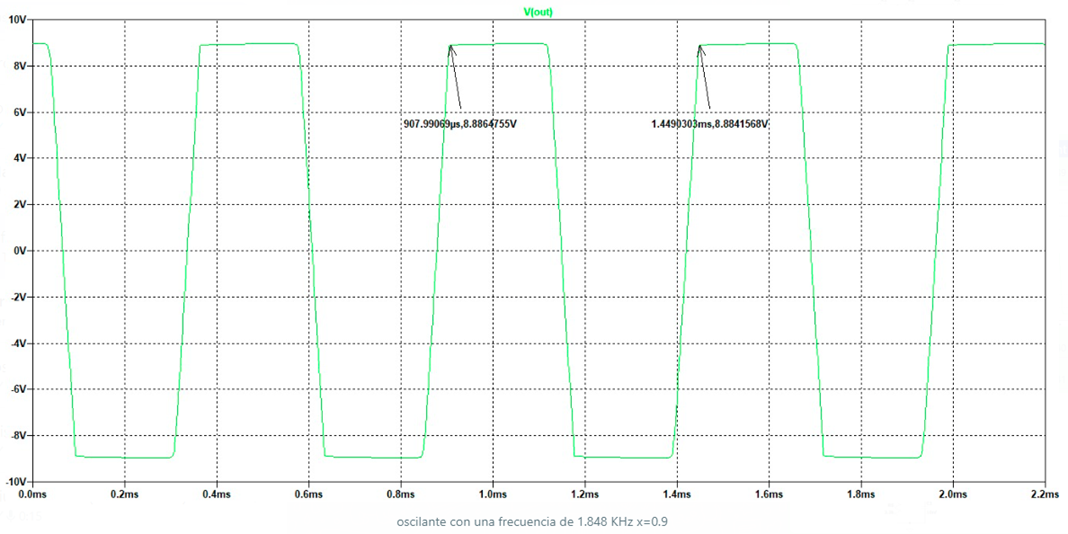
\includegraphics[width=15cm]{Imagenes/sim_puente_wien_sc9.png}
                        \caption{Simulación sin control de amplitud de la Figura \ref{fig:puente_wien_control} cuando X=0.10. Saturado}
                        \label{fig:sim_puente_wien_sc9}
                    \end{figure}

                    \begin{figure}[H]
                        \centering
                        \setcounter{figure}{8}
                        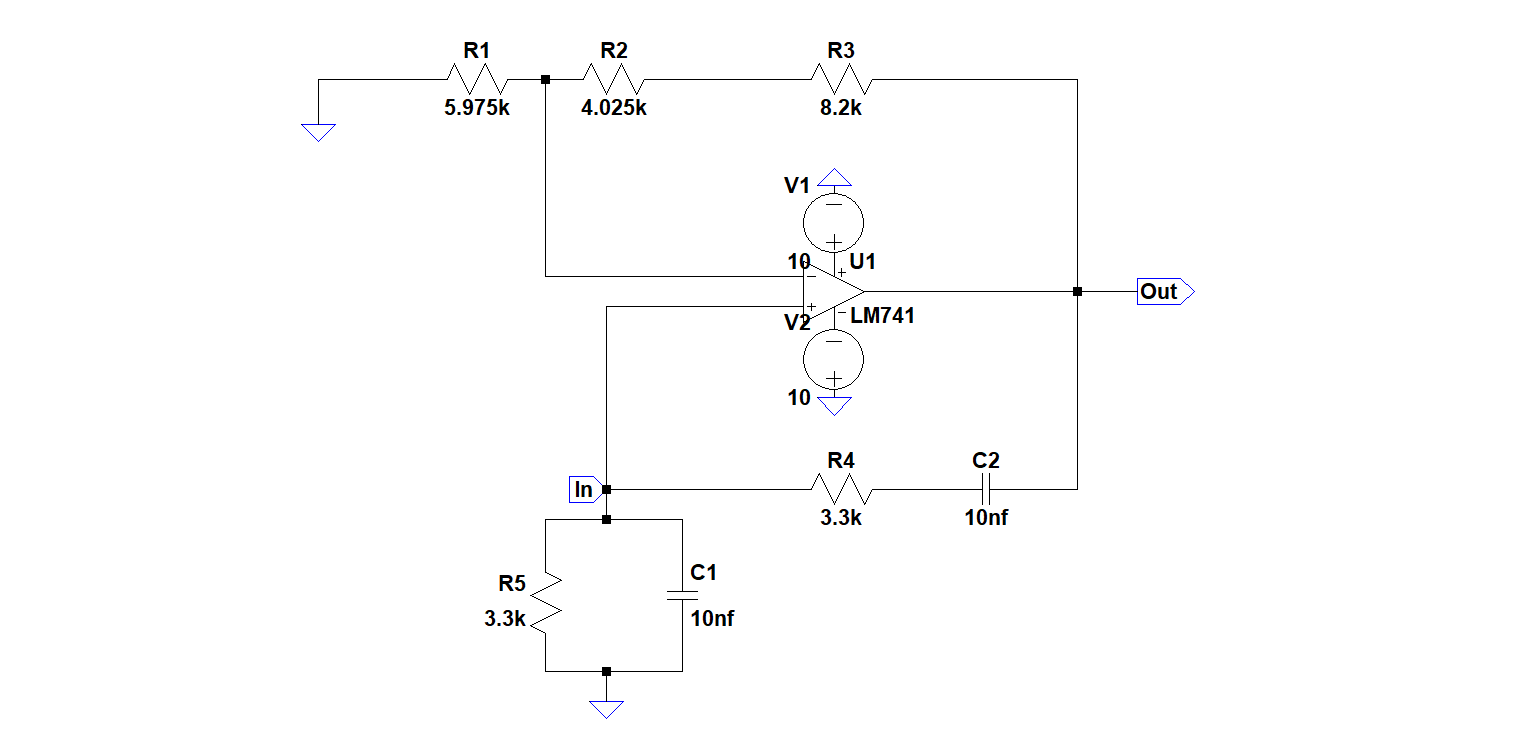
\includegraphics[width=10cm]{Imagenes/sim_cir_puente_wien_sc402.png}
                        \caption{Circuito sin control de amplitud de la Figura \ref{fig:puente_wien_control} cuando X=0.598.}
                        \label{fig:sim_cir_puente_wien_sc402}
                    \end{figure}

                    \begin{figure}[H]
                        \centering
                        \renewcommand{\figurename}{Gráfica}
                        \setcounter{figure}{4}
                        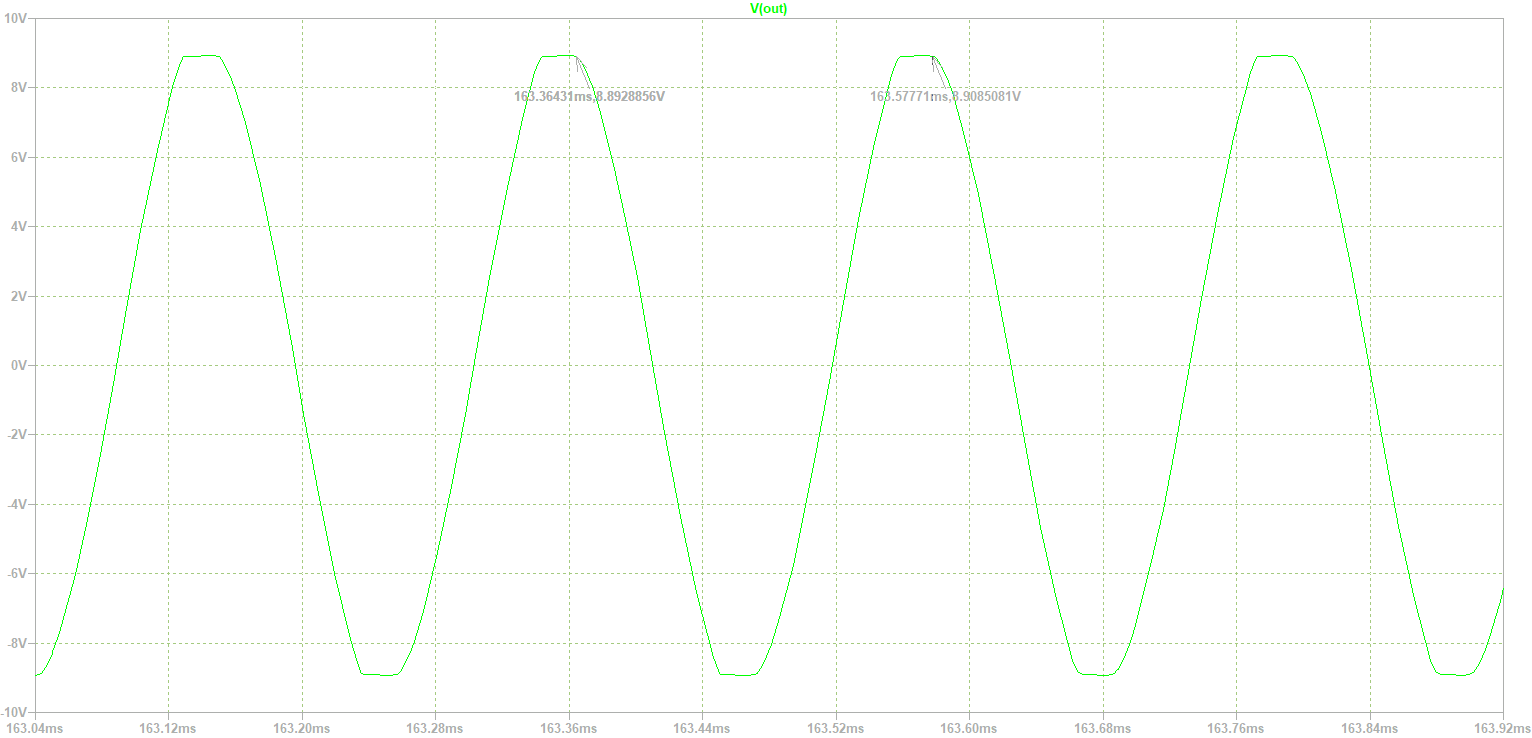
\includegraphics[width=15cm]{Imagenes/sim_puente_wien_sc402.png}
                        \caption{Simulación sin control de amplitud de la Figura \ref{fig:puente_wien_control} cuando X=0.598. Oscilando}
                        \label{fig:sim_puente_wien_sc402}
                    \end{figure}

                    Teniendo en cuenta cada una de las simulaciones realizadas, sus resultados mas importantes serán reflejados en la siguiente tabla:

                    \begin{table}[H]
                      \centering
                      \begin{tabular}{|c|c|c|c|}
                        \hline
                        \textbf{Estado} & $\mathbf{\text{T} [\mu s]}$ & \textbf{f [KHz]} & $\mathbf{XR_{v1} [\ohm]}$ \\
                        \hline
                        Inestable & - & - & $0.60\, (10 \, k)$ \\
                        \hline
                        Estable & $213.4$ & $4.69$ & $0.598\, (10 \, k)$ \\
                        \hline
                        Saturado & $240.38$ & $4.16$ & $0.50\, (10 \, k)$ \\
                        \hline
                        Saturado & $284.03$ & $3.52$ & $0.40\, (10 \, k)$ \\
                        \hline
                        Saturado & $540.54$ & $1.85$ & $0.10\, (10 \, k)$ \\
                        \hline
                      \end{tabular}
                      \caption{Mediciones tomadas tras las simulaciones de la Figura \ref{fig:puente_wien_control} sin control de amplitud.}
                      \label{tab:sim_puente_wien_sc}
                    \end{table}

                \item \textbf{Con Control de Amplitud} 

                     \begin{figure}[H]
                        \centering
                        \setcounter{figure}{9}
                        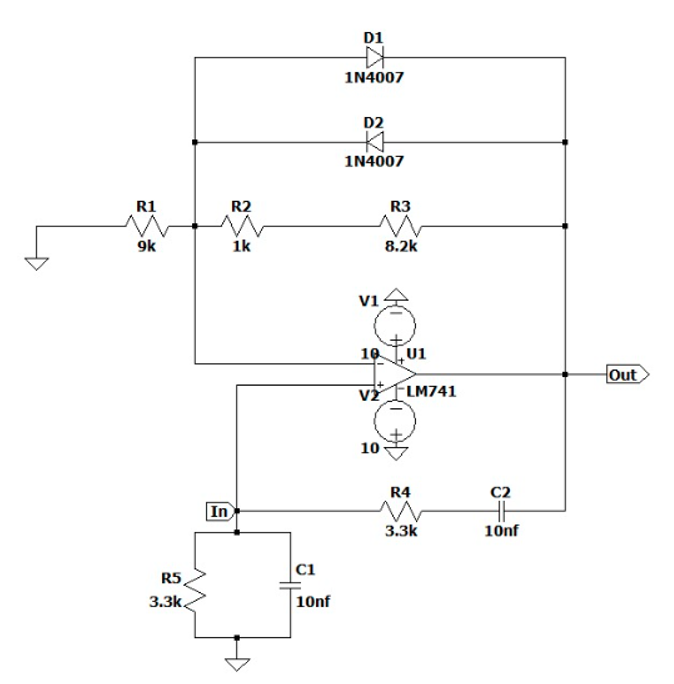
\includegraphics[width=8cm]{Imagenes/sim_cir_puente_wien_control0.png}
                        \caption{Circuito con control de amplitud de la Figura \ref{fig:puente_wien_control} cuando X=0.90.}
                        \label{fig:sim_cir_puente_wien_control0}
                    \end{figure}

                    \begin{figure}[H]
                        \centering
                        \renewcommand{\figurename}{Gráfica}
                        \setcounter{figure}{5}
                        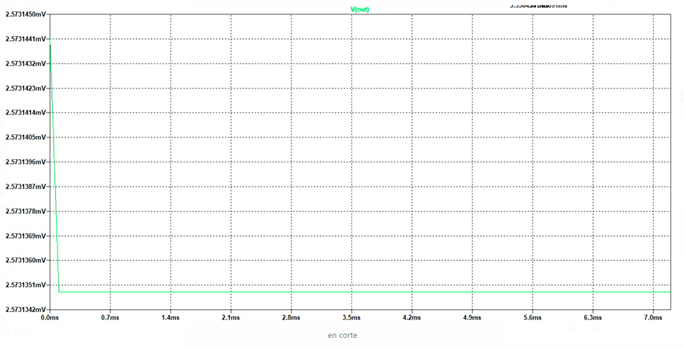
\includegraphics[width=15cm]{Imagenes/sim_puente_wien_control0.png}
                        \caption{Simulación con control de amplitud de la Figura \ref{fig:puente_wien_control} cuando X=0.90. Corte}
                        \label{fig:sim_puente_wien_control0}
                    \end{figure}
                    
                     \begin{figure}[H]
                        \centering
                        \setcounter{figure}{10}
                        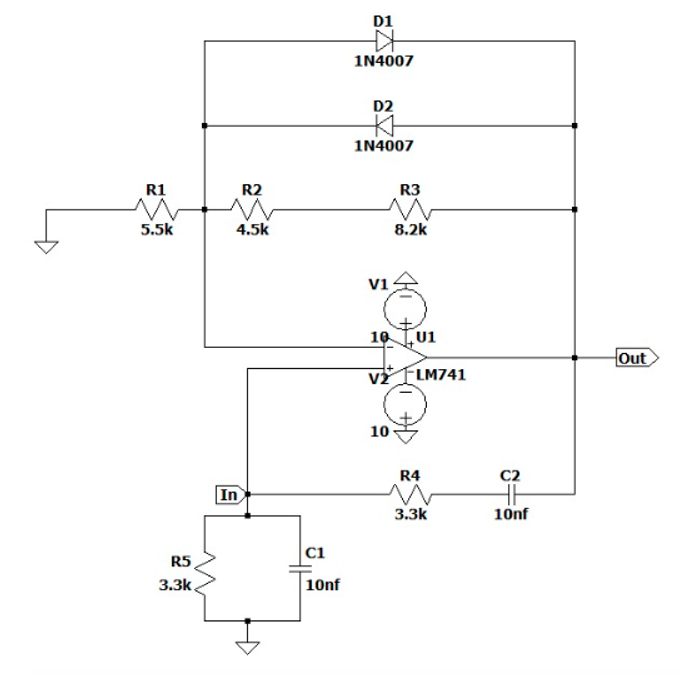
\includegraphics[width=8cm]{Imagenes/sim_cir_puente_wien_control45.png}
                        \caption{Circuito con control de amplitud de la Figura \ref{fig:puente_wien_control} cuando X=0.40.}
                        \label{fig:sim_cir_puente_wien_control45}
                    \end{figure}

                    \begin{figure}[H]
                        \centering
                        \renewcommand{\figurename}{Gráfica}
                        \setcounter{figure}{6}
                        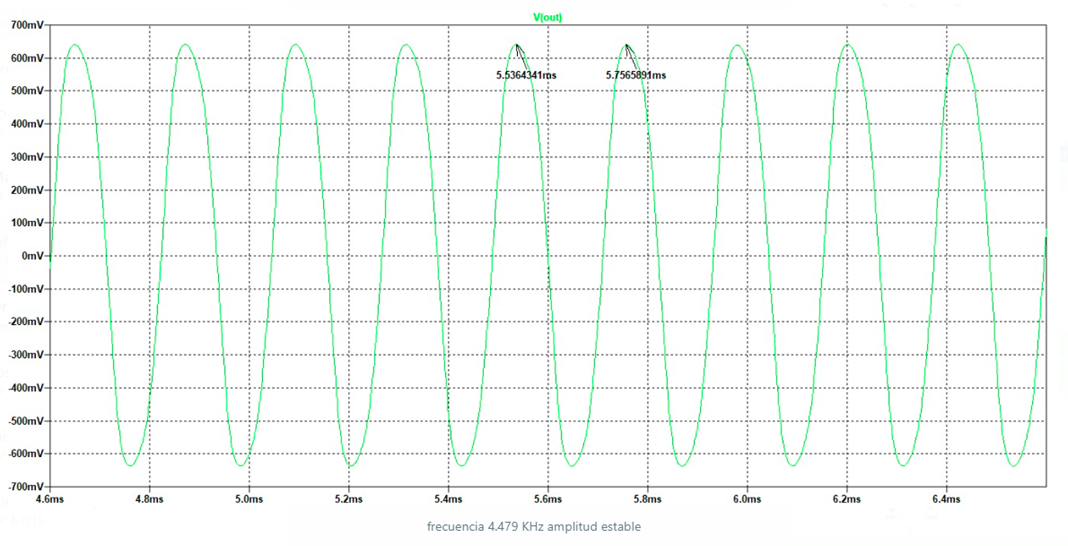
\includegraphics[width=15cm]{Imagenes/sim_puente_wien_control45.png}
                        \caption{Simulación con control de amplitud de la Figura \ref{fig:puente_wien_control} cuando X=0.40. Oscilando}
                        \label{fig:sim_puente_wien_control45}
                    \end{figure}
                    
                    
                    
                     \begin{figure}[H]
                        \centering
                        \setcounter{figure}{11}
                        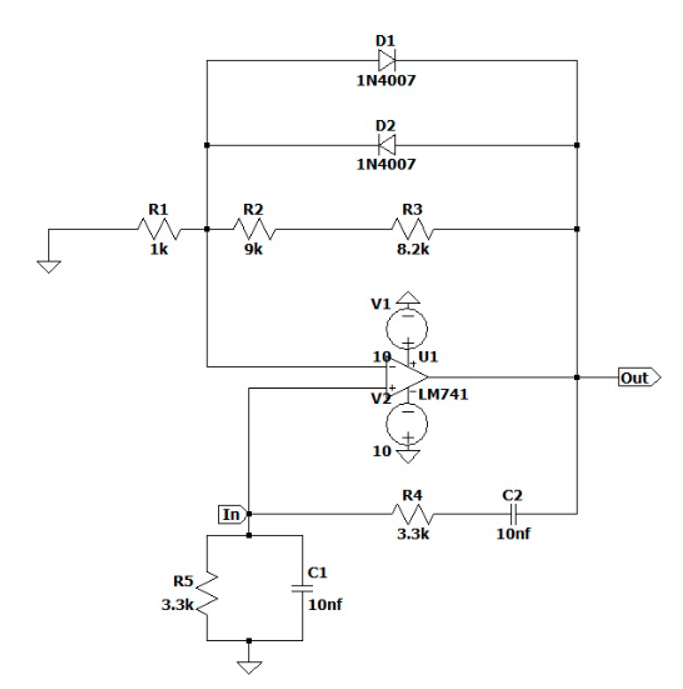
\includegraphics[width=8cm]{Imagenes/sim_cir_puente_wien_control9.png}
                        \caption{Circuito con control de amplitud de la Figura \ref{fig:puente_wien_control} cuando X=0.10.}
                        \label{fig:sim_cir_puente_wien_control9}
                    \end{figure}

                    \begin{figure}[H]
                        \centering
                        \renewcommand{\figurename}{Gráfica}
                        \setcounter{figure}{7}
                        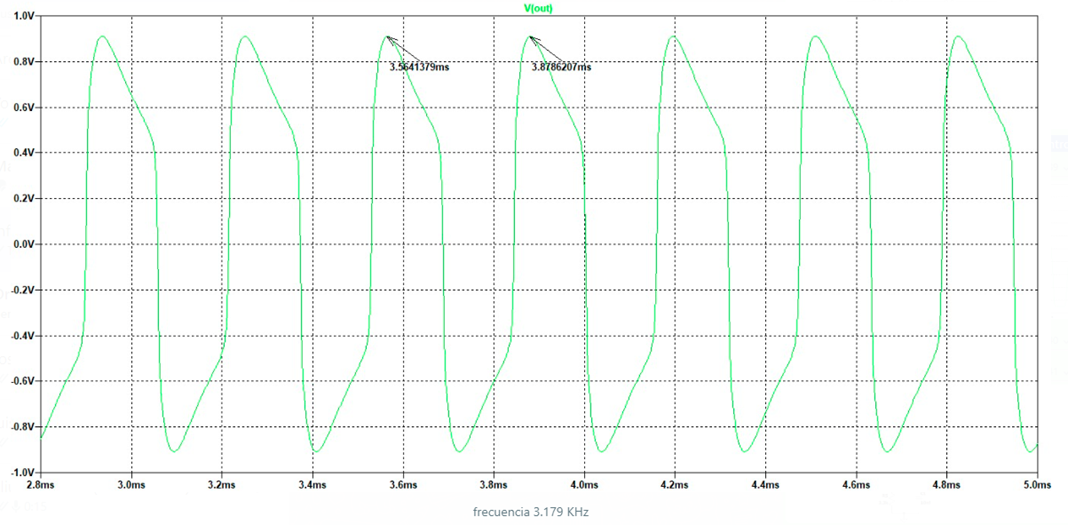
\includegraphics[width=15cm]{Imagenes/sim_puente_wien_control9.png}
                        \caption{Simulación con control de amplitud de la Figura \ref{fig:puente_wien_control} cuando X=0.10. Saturado}
                        \label{fig:sim_puente_wien_control9}
                    \end{figure}
                    
                    
                    Por ultimo, con las simulaciones realizadas se obtuvieron los siguientes datos, simplificando la visualización de estos últimos.

                    \begin{table}[H]
                      \centering
                      \begin{tabular}{|c|c|c|c|}
                        \hline
                        \textbf{Estado} & $\mathbf{\text{T} [\mu s]}$ & \textbf{f [kHz]} & $\mathbf{XR_{v1} [\ohm]}$ \\
                        \hline
                        Corte & - & - & $0.90 \, (10 \, k)$ \\
                        \hline
                        Oscilación & $223.26$ & $4.48$ & $0.40 \, (10 \, k)$ \\
                        \hline
                        Saturación & $314.46$ & $3.18$ & $0.10 \, (10 \, k)$ \\
                        \hline
                      \end{tabular}
                      \caption{Mediciones tomadas tras las simulaciones de la Figura \ref{fig:puente_wien_control} con control de amplitud.}
                      \label{tab:sim_puente_wien_control}
                    \end{table}

                    
            \end{itemize}
    \end{enumerate}

    
    \subsection{Parte 2. Multivibradores}\label{subsec:meto_parte2}

        \begin{figure}[H]
            \centering
            \setcounter{figure}{12}
            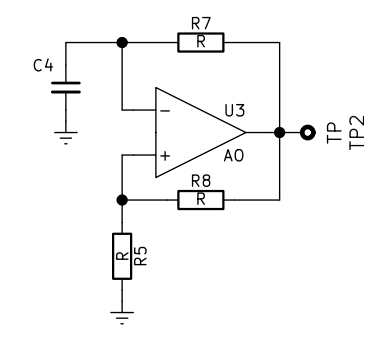
\includegraphics[width=8cm]{Circuitos/astable.png}
            \caption{Multivibrador astable con base en A.O.}
            \label{fig:astable}
        \end{figure}
        
     
        
        \begin{enumerate}

            \subsubsection{Diseño}
            \item Para el circuito de la figura \ref{fig:astable}, diseñe (especifique valores comerciales, para cada elemento) con el fin de obtener una oscilación de frecuencia 5;0 KHz y amplitud de 2 $V_pico$

                Donde, 
                $\mathbf{V_o}$:La salida del Amp. Op.         
                $\mathbf{V_c}$:Nodo de la entrada inversora del Amp. Op. o Voltaje del capacitor.         
                $\mathbf{V_p}$:Nodo de la entrada no inversora del Amp. Op.

                Hallando $V_p$, tenemos.

                \begin{gather}
                    V_p=\dfrac{R_5}{R_5+R_8}V_o \label{eqn:vp}
                \end{gather}

                Como se tiene retroalimentación positiva la salida $V_o$ va a tender a saturarse, teniendo una salida máxima positiva y negativa. Por lo tanto, tenemos lo siguiente:

                \begin{gather}
                    V_{omax}=V_{sat}^+ \label{eqn:vomax} \\[0.5cm]
                    V_{omin}=V_{sat}^- \label{eqn:vomin}                     
                \end{gather}

                Ahora hallando el voltaje del capacitor tenemos,

                \begin{gather}
                    V_f=V_o=V_{sat}^+=V_{R_7}+V_c \label{eqn:vsat+}\\[0.5cm]
                    V_{sat}^+=IR_7+V_c=R_7C_4\dfrac{dV_c}{dt}+V_c \quad \text{ordenando la siguiente ec. diferencial} \nonumber\\[0.5cm]
                    \dfrac{dV_c}{dt}+\dfrac{1}{R_7C_4}V_c=\dfrac{1}{R_7C_4}V_{sat}^+ \nonumber\\[0.5cm]
                    \text{Resolviendo esta ec. diferencial se tiene,} \nonumber\\[0.5cm]
                    V_c(t)=A+Be^{-\dfrac{t}{R_7C_4}} \label{eqn:vct}
                \end{gather}

                Ahora observando la siguiente gráfica \ref{fig:astable_sal_ent}, se hallan el Caso 1 y 2, de esa manera se encuentran las constantes de la ecuación \ref{eqn:vct}

                \begin{figure}[H]
                    \centering
                    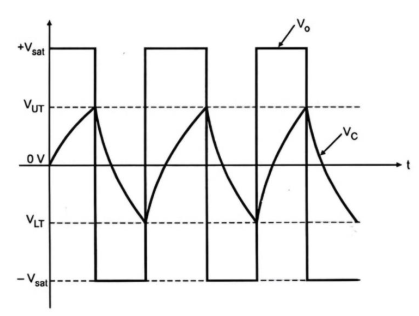
\includegraphics{Imagenes/astable_sal_ent.png}
                    \caption{Voltaje de salida (Vsat+) y del divisor de tensión (Vp)}
                    \label{fig:astable_sal_ent}
                \end{figure}

                Observando la Gráfica \ref{fig:astable_sal_ent} se realizará un estudio para hallar el tiempo en cada uno de sus tiempos de encendido (Caso 1) y apagado (Caso 2), 
                
                \begin{itemize}
            
                    \item      \textbf{Caso 1}

                        De la ecuación \ref{eqn:vct}, sustituiremos los siguientes valores de t
                        
                        $t=0$
                        \begin{gather}
                            \dfrac{R_5}{R_5+R_8}V_{sat}^-=A+B \label{eqn:a+b}
                        \end{gather}

                        $t=\infty$
                        \begin{gather}
                            V_{sat}^+=A \label{eqn:a}
                        \end{gather}

                        Por lo tanto, el valor que obtenemos en B sustituyendo la ecuación \ref{eqn:a} en \ref{eqn:a+b} se obtiene lo siguiente:

                        \begin{gather}
                            B=\dfrac{R_5}{R_5+R_8}V_{sat}^--V_{sat}^+ \label{eqn:b} \\[0.5cm]
                            \text{Sustituyendo las ecuaciones \ref{eqn:a} y \ref{eqn:b} en la ecuación \ref{eqn:vct} se tiene,}  \nonumber\\[0.5cm]
                            V_c(t)=V_{sat}^++\left(\dfrac{R_5}{R_5+R_8}V_{sat}^--V_{sat}^+\right)e^{-\dfrac{t}{R_7C_4}}  \label{eqn:vct2}
                        \end{gather}

                        Sustituyendo la ecuación \ref{eqn:vc2} en la ecuación \ref{eqn:vct2}, siendo el valor del caso 1, teniendo en cuenta que lo siguiente que se va desarrollar, tiene que ver con que los nodos de cada entrada, tomando el amplificador como ideal, poseen el mismo valor de voltaje, Por esa razón,

                        \begin{gather}
                            V_c=V_p^+=\dfrac{R_5}{R_5+R_8}V_{sat}^+ \label{eqn:vc2}
                        \end{gather}

                        \begin{gather}
                            \dfrac{R_5}{R_5+R_8}V_{sat}^+ = V_{sat}^++\left(\dfrac{R_5}{R_5+R_8}V_{sat}^--V_{sat}^+\right)e^{-\dfrac{t_1}{R_7C_4}} \label{eqn:t}
                        \end{gather}

                        Despejando $t_1$, se tiene.

                        \begin{gather}
                            ln\left(e^{-\dfrac{t_1}{R_7C_4}}\right)=ln\left(\dfrac{\dfrac{R_5}{R_5+R_8}V_{sat}^+-V_{sat}^+}{\dfrac{R_5}{R_5+R_8}V_{sat}^--V_{sat}^+}\right) \nonumber \\[0.5cm]
                            t_1=-R_7C_4ln\left(\dfrac{\dfrac{R_5}{R_5+R_8}V_{sat}^+-V_{sat}^+}{\dfrac{R_5}{R_5+R_8}V_{sat}^--V_{sat}^+}\right) \label{eqn:t1}
                        \end{gather}

                    \item \textbf{Caso 2}

                        Debido a la simetría de la gráfica \ref{fig:astable_sal_ent}, $t_1=t_2$, desarrollando se puede hallar su periodo.

                        \begin{gather}
                            T=t_1+t_2=2 \, t_1=-2R_7C_4ln\left(\dfrac{\dfrac{R_5}{R_5+R_8}V_{sat}^+-V_{sat}^+}{\dfrac{R_5}{R_5+R_8}V_{sat}^--V_{sat}^+}\right) \label{eqn:T}
                        \end{gather}

                        Siendo la frecuencia el inverso del periodo,

                        \begin{gather}
                            f=\dfrac{1}{T} \label{eqn:f}
                        \end{gather}

                        Teniendo la ecuación \ref{eqn:T} se obtiene lo siguiente para simplificar,

                        \begin{gather}
                            V_{sat}^+=-V_{sat}^- \text{Sustituyendo esta ecuación en \ref{eqn:T}} \nonumber \\[0.5cm]
                            T=t_1+t_2=2 \, t_1=-2R_7C_4ln\left(\dfrac{\dfrac{R_5}{R_5+R_8}V_{sat}^+-V_{sat}^+}{\dfrac{R_5}{R_5+R_8}(-V_{sat}^+)-V_{sat}^+}\right) \nonumber \\[0.5cm]
                            T=-2R_7C_4 ln\left(\dfrac{V_{sat}^+\left(\dfrac{R_5}{R_5+R_8}-1\right)}{-V_{sat}^+\left(\dfrac{R_5}{R_5+R_8}+1\right)}\right) \nonumber \\[0.5cm]
                            T=-2R_7C_4 ln\left(\dfrac{R_5-R_5-R_8}{-(R_5+R_5+R_8)}\right)\nonumber \\[0.5cm]
                            T=-2R_7C_4 ln\left(\dfrac{R_8}{2R_5+R_8}\right) \label{eqn:T2}
                        \end{gather}

                        Ahora se tiene que la amplitud esta dada por la ecuación \ref{eqn:vc2}, tomando en cuenta el voltaje swing del Amp. Op. que se halla en el datasheet, que se encuentra en la sección \ref{sec:anexos}.

                        Posee un valor de $V_{swingAO}=1.5V$. Por lo tanto, $V_{sat}^+$ y $V_{sat}^-$  se observan de la siguiente manera:

                        \begin{gather}
                            V_{sat}^+=V_{CC}-V_{swingAO} \label{eqn:vsat2}
                        \end{gather}

                        Para que se cumpla  $V_{sat}^+=-V_{sat}^-$, se debe cumplir,
                        $V_{CC}=-V_{EE}$.

                        Si alimentamos con 10V, se desarrolla lo siguiente;

                        \begin{gather}
                            V_{sat}^+=10-1.5=8.5 \, V \label{eqn:vsatultimo} \\[0.5cm]
                            V_{sat}^-=-V_{sat}^+=-8.5 \, V \label{eqn:vsatultimo2}
                        \end{gather}

                        Lo deseado en el diseño es que su amplitud seaa $2V_{pico}$, por consiguiente, se sustituyen las ecuaciones \ref{eqn:vsatultimo} en \ref{eqn:vc2}

                        \begin{gather}
                            2=\dfrac{R_5}{R_5+R_8}(8.5V) \Rightarrow \dfrac{2}{8.5}=\dfrac{4}{17}=\dfrac{R_5}{R_5+R_8} \nonumber \\[0.5cm]
                            4R_5+4R_8=17R_5 \Rightarrow 4R_8=13R_5 \nonumber \\[0.5cm]
                            R_8=\dfrac{13}{4}R_5=3.25R_5 \approx 3R_5 \nonumber \\[0.5cm]
                            R_8=3R_5 \label{eqn:r8}
                        \end{gather}

                        Podemos asumir que $R_5=1k \ohm$ y $R_8=3.3k \ohm$

                        Sustituyendo \ref{eqn:r8} en la ecuación \ref{eqn:T2}, por lo tanto,

                        \begin{gather}
                            T=-2R_7C_4ln\left(\dfrac{3R_5}{2R_5+3R_5}\right)=-2R_7C_4ln\left(\dfrac{3R_5}{5R_5}\right) \nonumber \\[0.5cm]
                            T=-2R_7C_4ln\left(\dfrac{3}{5}\right) \label{eqn:T3}
                        \end{gather}

                        Asumiendo $C_4=10 \, nF$, podemos hallar $R_7$, para una frecuencia de 5 KHz o un periodo de $T=0.2 \, ms$, sustituyendo en la ecuación \ref{eqn:T3} despejamos $R_7$.

                        \begin{gather}
                            R_7=\dfrac{T}{-2C_4ln\left(\dfrac{3}{5}\right) }=\dfrac{0.2 ms}{-2(10n)ln\left(\dfrac{3}{5}\right)}=19.58 K \ohm        
                        \end{gather}

                        El valor comercial cercano es $R_7=18 k\ohm$

                                            
                \end{itemize}

            
            \item Para el circuito de la figura \ref{fig:monoestable}, diseñe (especifique valores comerciales, para cada elemento) con el fin de obtener un tiempo de pulso de 10ms. Indique las características de la señal de disparo, la frecuencia máxima a la que este puede repetirse y la factibilidad de obtenerla en el laboratorio.

                \begin{figure}[H]
                    \centering
                    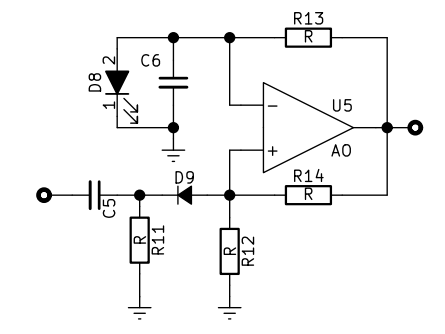
\includegraphics[width=10cm]{Circuitos/monoestable.png}
                    \caption{Multivibrador monoestable con base en A.O.}
                    \label{fig:monoestable}
                \end{figure}
            
                Tomando en cuenta la figura \ref{fig:monoestable}, para poder realizar un análisis previo a los cálculos del diseño se tiene lo siguiente, al inyectar una señal de entrada $V_i \geq 0V$, el mismo circuito se comportará como un multivibrador astable, esto debido a la polarización del diodo D9 con la diferencia que la tensión del capacitor C6 e mantendrá estable cuando $V_{D8}=V_{C6}$, además el $V_{D8}$ debe ser menor a $V_p^+$, ocasionando que este oscile. De esa manera, tenemos $V_{D8}<V_p^+$.

                Ahora si  se excita el circuito con un pulso negativo en la entrada el diodo D9 conducirá, además el capacitor C5 se carga con un valor negativo, por tanto, el $V_p$ disminuya bruscamente en un instante y así haciendo que la entrada inversora sea mayor que la no inversora, más el capacitor C6 inicia a descargarse hasta el punto que la no inversora se vuelva más alta y se vuelve a estabilizar como un astable con la tensión del capacitor C6 limitada por el diodo D8, esto hasta que en la entrada se vuelva a excitar el circuito con un pulso negativo, repitiendo el ciclo.

                Por ende, podemos ahora indicar el análisis circuital realizado, como se indico se mantiene en un caso especifico como un multivibrador estable, debido a esto podemos usar la ecuación \ref{eqn:t1}, sin embargo, primero se asumirá el voltaje de salida del amplificador como un voltaje positivo, para este caso el voltaje en el nodo $V_p$ vendrá dado por la ecuación \ref{eqn:vp}, con sus valores correspondientes 

                \begin{gather}
                    V_{p2}=\dfrac{R_{12}}{R_{12}+R_{14}}V_{Omax} \label{eqn:vp2}
                \end{gather}

                Ahora si visualizamos la caída de tensión en $R_11$ que denotaremos como $V_{p3}$, en este caso, de lo antes mencionado, D9 no conduce, durante este caso el condensador C6 se cargara hasta el voltaje D8, por tanto $V_{P1}>V_{D8}$, eso hará que la salida se mantenga estable en $V_{Omax}$. Ahora si se introduce una señal negativa en la entrada de valor –Vi, D9 conducirá, obteniendo

                \begin{gather}
                    V_{p3}=-V_i+V_{D9} \label{vp3}
                \end{gather}

                Justo en el momento ese momento $V_{P3}<V_{D8}$ por lo tanto la salida cambia a ser $V_{Omin}$ y $V_p$ pasara a ser
                
                \begin{gather}
                    V_{p3}=\dfrac{R_{12}}{R_{12}+R_{14}}V_{Omin} \label{eqn:vp3}
                \end{gather}

                Ahora, tomando en cuenta el intervalo t1 y sabiendo que el voltaje del condensador vendrá dado por la ecuación \ref{eqn:t1}, llevándolo a sus expresión del $V_{Omin}$

                \begin{gather}
                    t_1=-R_{13}C_6ln\left(\dfrac{\left(\dfrac{R_{12}}{R_{12}+R_{14}}-1\right)V_{Omin}}{\dfrac{R_{12}}{R_{12}+R_{14}}V_{Omax}-V_{Omin}}\right) \label{eqn:t2}
                \end{gather}
                
                Pero también sabemos que $V_{P2}$ es igual al voltaje del diodo D8 por lo que nos queda,

                \begin{gather}
                    t_1=-R_{13}C_6ln\left(\dfrac{\left(\dfrac{R_{12}}{R_{12}+R_{14}}-1\right)V_{Omin}}{V_{D8}-V_{Omin}}\right) \label{eqn:t3}
                \end{gather}

                Tomando en cuenta el resultado \ref{eqn:r8}, en este caso $R_{14}=3R_{12}$, desarrollando lo anterior tenemos,

                \begin{gather}
                    t_1=-R_{13}C_6ln\left(\dfrac{\left(-\dfrac{3}{4}\right)V_{Omin}}{V_{D8}-V_{Omin}}\right) \nonumber
                \end{gather}
            
                Siendo $V_{D8}=1.6V$ por ser un Led rojo y un $V_{Omin}=-8.5V$ y se quiere que el pulso dure 10ms se tiene,

                \begin{gather}
                    10m=-2R_{13}(10n)ln\left(\dfrac{\left(-\dfrac{3}{4}\right)(-8.5)}{1.6-(-8.5)}\right) \nonumber\\[0.5cm]
                    \text{Despejando $R_{13}$} \nonumber\\[0.5cm]
                    R_{13}=\dfrac{10m}{2(10n)ln(0.632)}=1.087 \, M\ohm \approx 1 \, M \ohm \label{eqn:r13}
                \end{gather}


            \subsubsection{Simulación}
            
            \item Simule el circuito diseñado de la figura \ref{fig:astable} (astable) y verifique las especificaciones, reporte además las formas de onda de interés para evidenciar el funcionamiento del circuito.

                \begin{figure}[H]
                    \centering
                    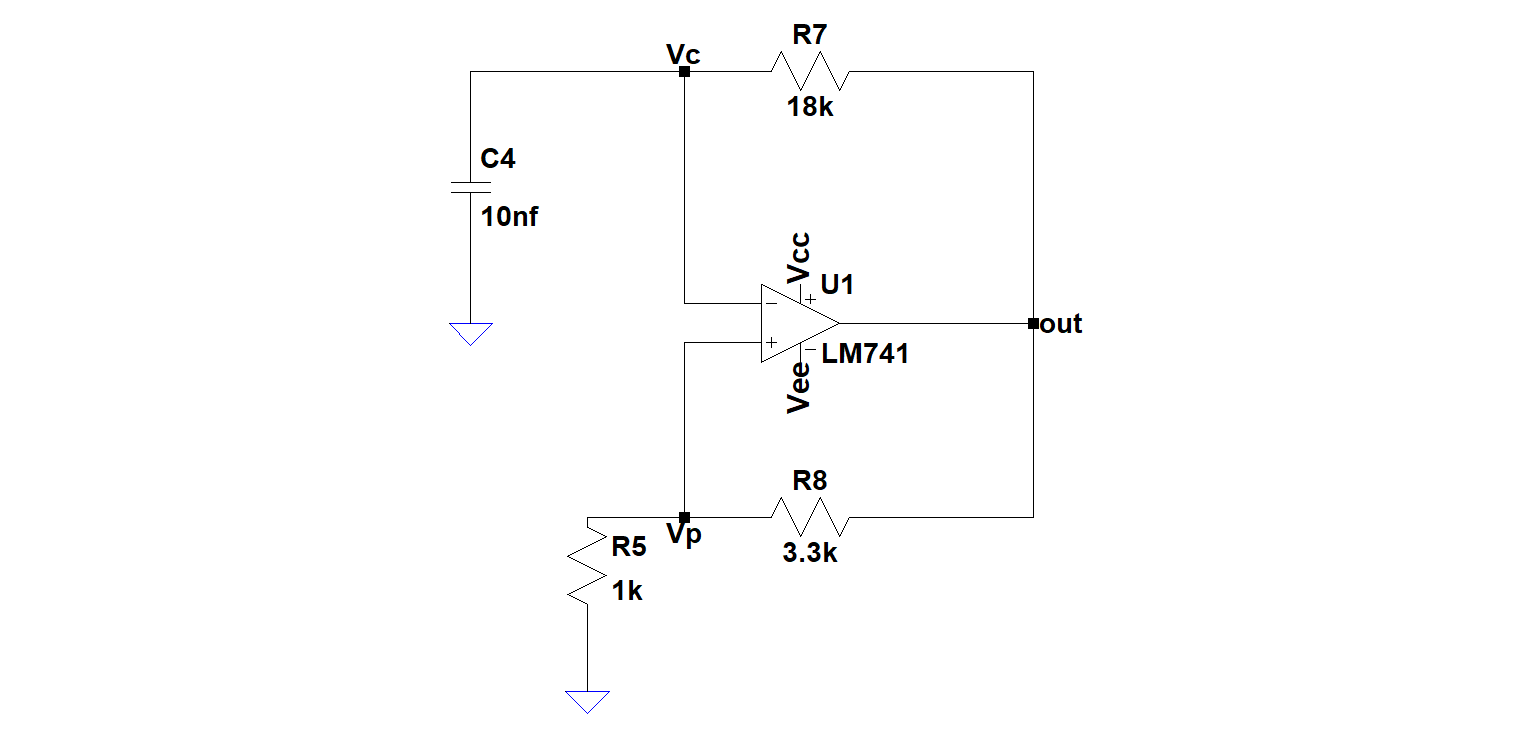
\includegraphics[width=10cm]{Circuitos/sim_cir_astable.png}
                    \caption{Diseño del Multivibrador Astable usado en la simulación}
                    \label{fig:sim_cir_astable}
                \end{figure}

                \begin{figure}[H]
                    \centering
                    \renewcommand{\figurename}{Gráfica}
                    \setcounter{figure}{8}
                    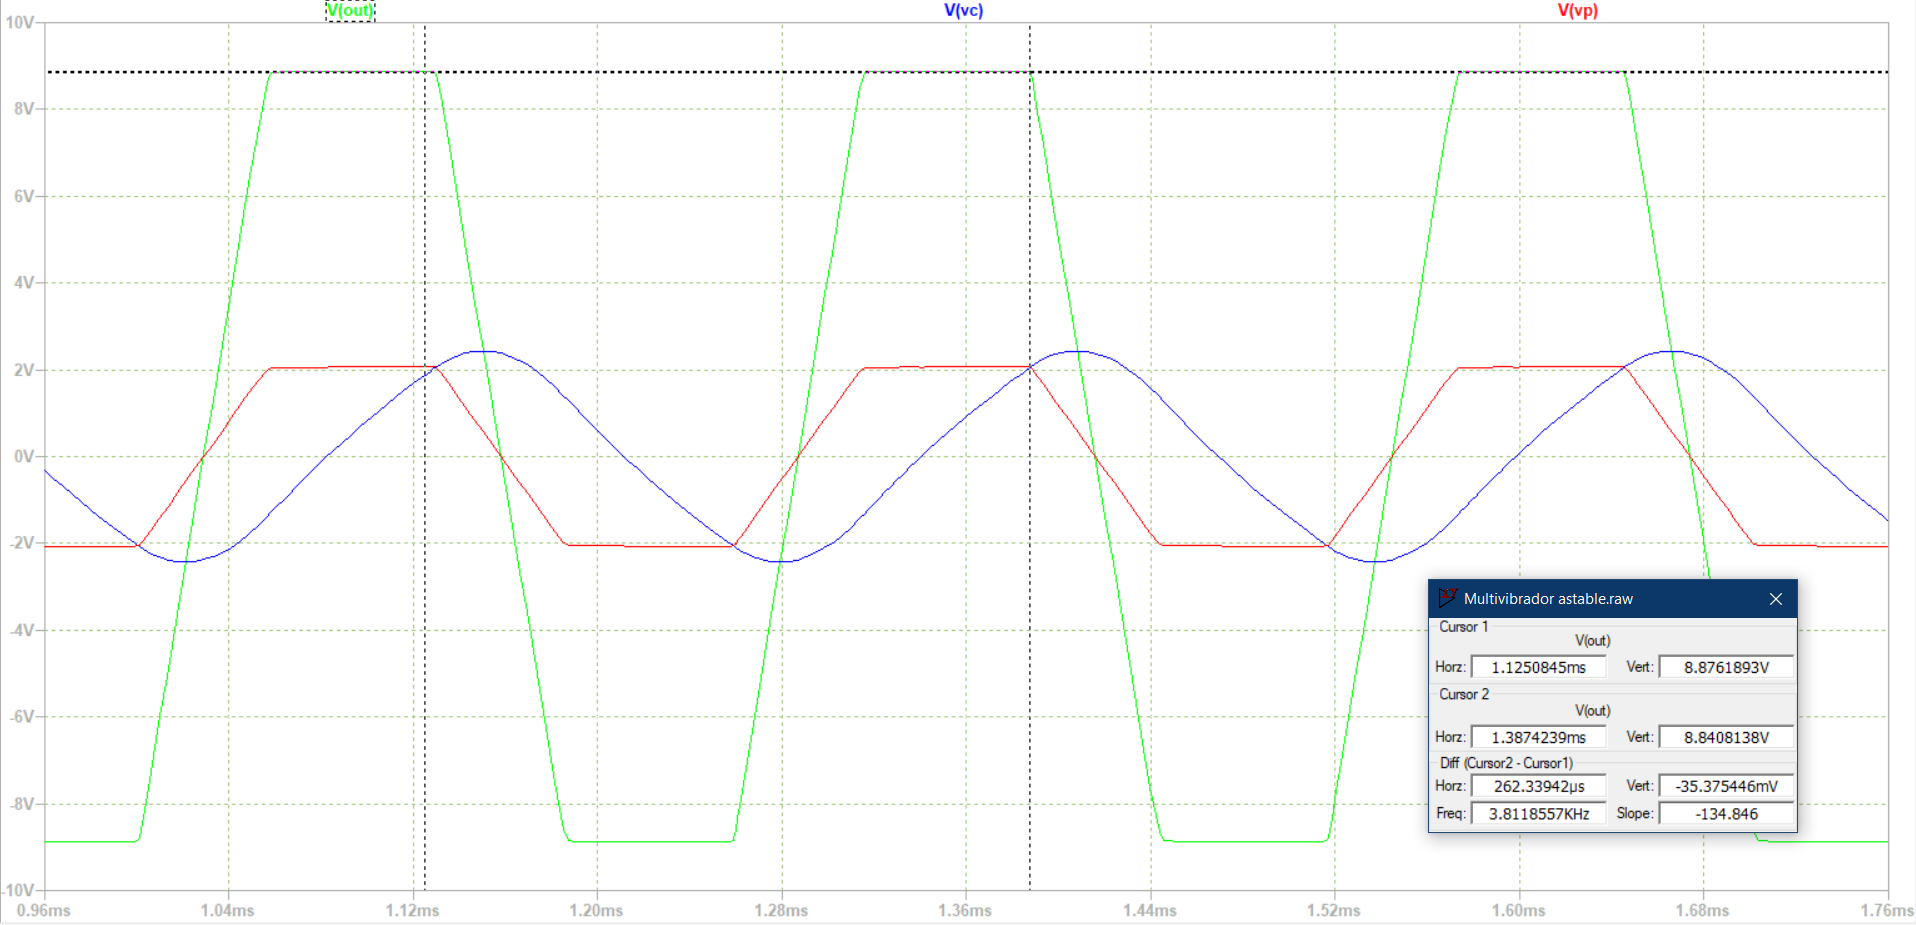
\includegraphics[width=10cm]{Imagenes/sim_astable.png}
                    \caption{Señal de salida de capacitor (Vc), del divisor de tensión (Vp) y la salida en general (Vout) del Multivibrador Astable en la simulación}
                    \label{fig:sim_astable}
                \end{figure}

                Como se puede observar cada salida en especial las de $V_{(vp)}$ y $V_{(out)}$ ambos están saturados que era lo esperado y quien termino generando una señal estable es la del capacitor siendo esta parecida a una sinusoidal, sin embargo en el diseño tuvimos un error con respecto a la frecuencia, debido a que se obtuvo una frecuencia de 3.81 KHz, y la adecuada era de 5 KHz, esta frecuencia nos hubiese permitido ver una señal en Vc triangular.

                
            
            \item Simule el circuito diseñado de la figura \ref{fig:monoestable} (monoestable) y verifique las especificaciones, el tiempo de pulso y el tiempo de recuperación. Reporte además las formas de onda de interés para evidenciar el funcionamiento del circuito.

                \begin{figure}[H]
                    \centering
                    \setcounter{figure}{16}
                    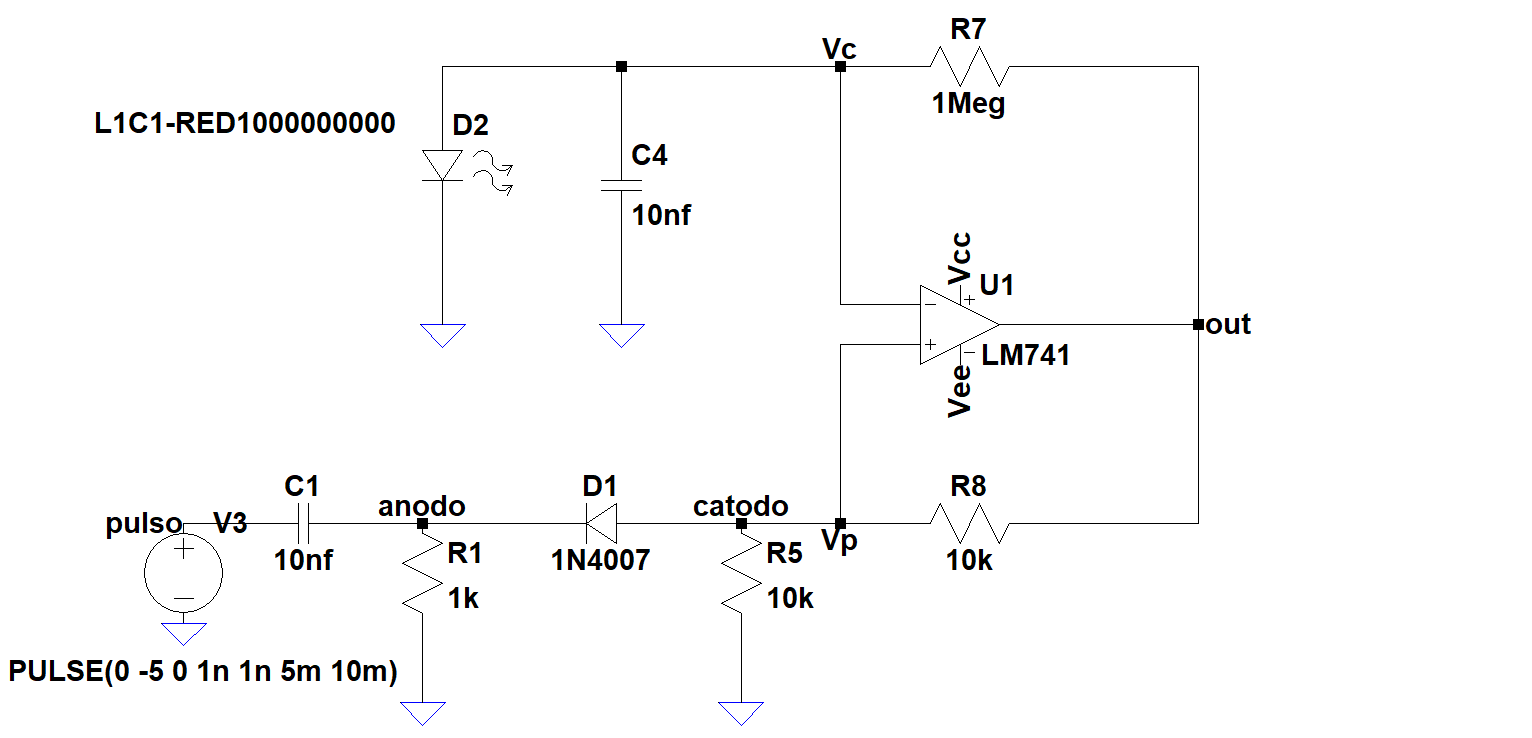
\includegraphics[width=10cm]{Circuitos/sim_cir_monoestable.png}
                    \caption{Diseño del Multivibrador Monoestable usado en la simulación}
                    \label{fig:sim_cir_monoestable}
                \end{figure}

                \begin{figure}[H]
                    \centering
                    \renewcommand{\figurename}{Gráfica}
                    \setcounter{figure}{9}
                    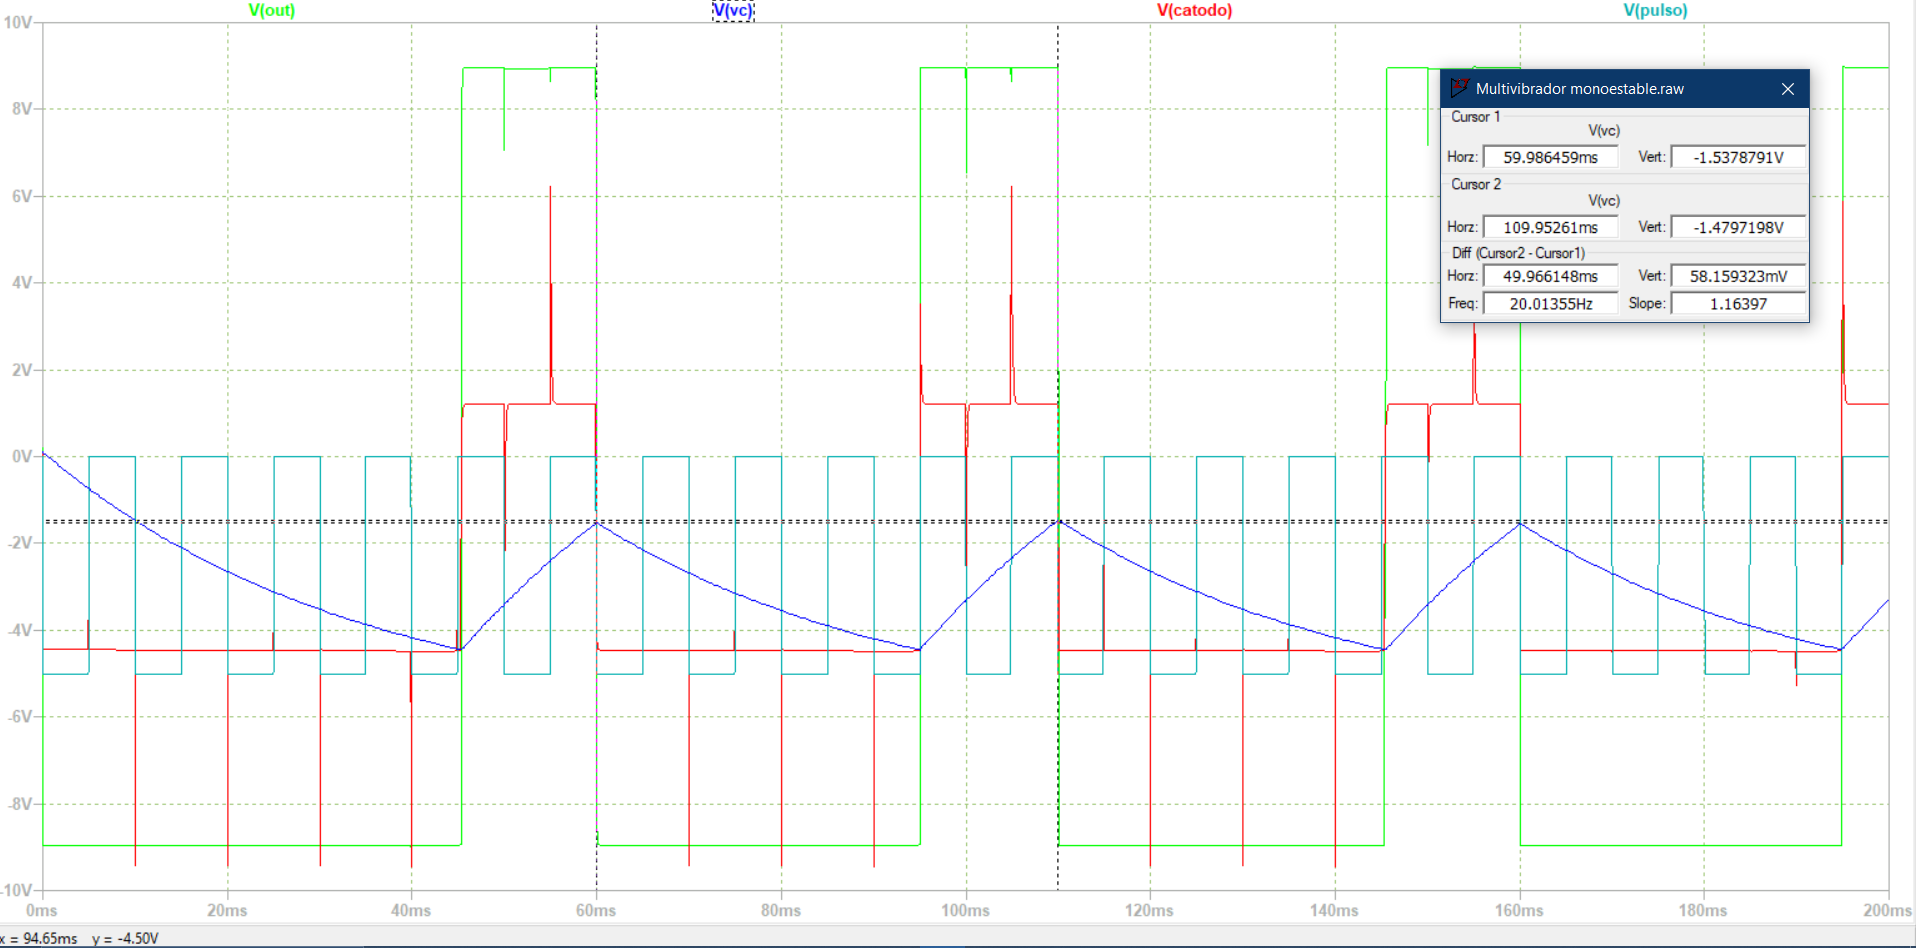
\includegraphics[width=10cm]{Imagenes/sim_monoestable.png}
                    \caption{Simulación del circuito \ref{fig:sim_cir_monoestable} donde V(out):Voltaje de salida,  V(vc):voltaje del capacitor limitado por el led, V(cátodo): voltaje del cátodo para observar su caída de tensión y V(pulso) el pulso negativo de entrada}
                    \label{fig:sim_monoestable}
                \end{figure}

                








            
        \end{enumerate}

    \subsection{Parte 3. Generador de Funciones} \label{subsec:met_parte3}

         \begin{figure}[H]
            \centering
            \setcounter{figure}{17}
            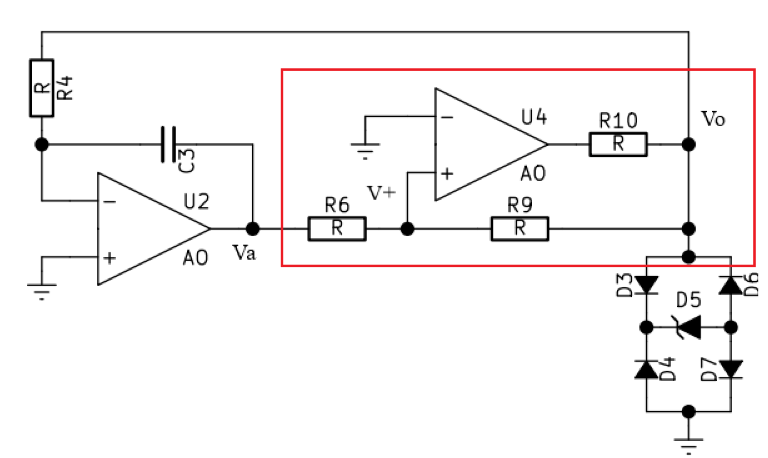
\includegraphics[width=8cm]{Circuitos/gf.png}
            \caption{Generador de funciones}
            \label{fig:gf}
        \end{figure}

        \begin{enumerate}
            \subsubsection{Diseño}
            \item Para el circuito de la figura \ref{fig:gf}, diseñe (especifique valores comerciales, para cada elemento) con el fin de obtener una oscilación de frecuencia 5.0 KHz. Utilice diodos zener con tensión zener por debajo de 7V

                En el circuito de la figura \ref{fig:gf} tenemos un generador de onda triangular y un generador de onda cuadrada. Tiene dos bloques bien definidos: el bloque conformado por el amplificador U4 (cuadro color rojo) es un comparador con histéresis, el bloque conformado por el amplificador U2 (externo al cuadro exceptuando los diodos) es un integrador. 
                
                El funcionamiento del generador es el siguiente, cuando se activa el circuito, la salida $V_o$ estará saturada. Supongamos que en primer lugar $V_o=V_{sat}^+$. Ahora este valor es la entrada del integrador, el cual produciría en la salida la ecuación de una recta con pendiente negativa (por ser inversor). En el instante inicial, la entrada inversora del amplificador U4 es nula y la entrada no inversora toma un valor positivo. Este último comenzaría a variar en función de la salida de integrador, el cual se estará haciendo más negativo a medida que transcurre el tiempo. Llega un punto en que la tensión en el puerto no inversor del amplificador U4 es más negativa que el voltaje en el puerto inversor, y la salida de este amplificador ahora será $V_o=V_{sat}^-$ . El proceso en el segundo semi ciclo es similar al anterior, sólo que este caso la pendiente de la recta es positiva. 
                
                Dicho esto, se puede definir de forma genérica el valor de tensión en el nodo $V^+$, correspondiente al puerto no inversor del amplificador U4.

                \begin{gather}
                    V^+=\dfrac{R_6}{R_6+R_9}V_o+\dfrac{R_9}{R_9+R_6}V_a \label{eqn:v+}
                \end{gather}

                Por otro lado, definimos la ecuación del integrador de la siguiente manera:

                \begin{gather}
                    V_a=-\dfrac{1}{SC_3R_4}V_o \Rightarrow SV_a=\dfrac{1}{C_3R_4}V_o \label{sva}
                \end{gather}

                Lo cual se puede expresar en el dominio del tiempo como,

                \begin{gather}
                    \dfrac{\partial V_a}{\partial t}=-\dfrac{1}{R_4C_3}V_o \Rightarrow \partial{V_a}=-\dfrac{1}{R_4C_3}V_o\partial t \nonumber \\[0.5cm]
                    \int_{V_o}^{V_f}\partial V_a=-\dfrac{1}{R_4C_3}V_o \int_{t_i}^{t_f}\partial t \Rightarrow V_f-V_i=-\dfrac{1}{R_4C_3}V_o (t_f-t_i) \label{eqn:dif_vyt}
                \end{gather}

                Ahora se define el valor umbral superior ($V_{us}$) e inferior ($V_{ui}$) de la oda triangular, evaluando en la ecuación \ref{eqn:v+}

                \begin{figure}[H]
                    \centering
                    \renewcommand{\figurename}{Gráfica}
                    \setcounter{figure}{10}
                    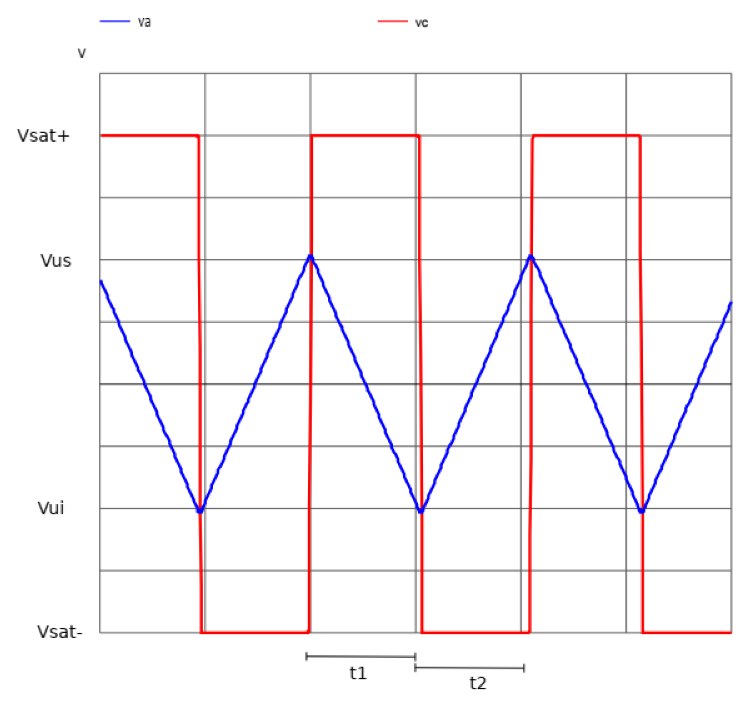
\includegraphics[width=10cm]{Imagenes/onda_gf.png}
                    \caption{Formas de onda en el generador}
                    \label{fig:ondas_gf}
                \end{figure}

                En la figura \ref{fig:ondas_gf} se puede observar el comportamiento gráfico del generador. Al evaluar la ecuación para $V^+=0$ para el instante $t_1$, es decir, en el instante en que va a cambiar el voltaje de salida por acción del comparador, se obtiene.

                \begin{gather}
                    0=\dfrac{R_6}{R_6+R_9}V_{sat}^++\dfrac{R_9}{R_6+R_9}V_{ui} \nonumber \\[0.5cm]
                    V_{ui}=-\dfrac{R_6}{R_9}V_{sat}^+ \label{eqn:vui} \\[0.5cm]
                    \text{Análoga para $t_2$ } \nonumber\\[0.5cm]
                    V_{us}=-\dfrac{R_6}{R_9}V_{sat}^- \label{eqn:vus} 
                \end{gather}

                Tomando en cuenta que $R_6<R_9$ para que sea menor los voltajes umbrales al de $V_{sat}$ para que no se saturen.

                De esta manera, se obtiene los valores umbrales de voltaje relacionado a los voltajes de alientación del integrador: $$V_{sat}^+ \quad \text{y} \quad V_{sat}^+$$

                Ahora, vamos a evaluar la ecuación \ref{eqn:dif_vyt}. Empezamos evaluando para el instante $t_1$, y obtenemos:

                \begin{gather}
                    V_{ui}-V_{us}=-\dfrac{1}{R_4C_3}V_{sat}^+t_1 \nonumber \\[0.5cm]
                    \text{Despejando $t_1$} \nonumber \\[0.5cm]
                    t_1=-\dfrac{(V_{ui}-V_{us})R_4C_3}{V_{sat}^+}=-\dfrac{R_4C_3\left[-\dfrac{R_6}{R_9}V_{sat}^+-\left(-\dfrac{R_6}{R_9}V_{sat}^-\right)\right]}{V_{sat}^+} \nonumber \\[0.5cm]
                    V_{sat}^-=-V_{sat}^+ \quad \therefore \nonumber \\[0.5cm]
                    t_1=R_4C_3\dfrac{\dfrac{R_6}{R_9}(V_{sat}^+-[-V_{sat}^+])}{V_{sat}^+}=\dfrac{R_4C_3R_62V_{sat}^+}{R_9V_{sat}^+} \nonumber \\[0.5cm]
                    t_1=2\dfrac{R_6}{R_9}R_4C_3 \label{eqn:t1_parte3}
                \end{gather}

                Analogamente, se encuentra el valor de $t_2$.

                \begin{gather}
                    t_2=2\dfrac{R_6}{R_9}R_4C_3 \label{eqn:t2_parte3}
                \end{gather}

                De esta manera, que la frecuencia del circuito es,

                \begin{gather}
                    T=t_1+t_2 \quad ; \quad t_1=t_2  \quad \therefore \nonumber \\[0.5cm]
                    T=2t_1=2\left[2\dfrac{R_6}{R_9}R_4C_3 \right] \nonumber \\[0.5cm]
                    T=4\dfrac{R_6}{R_9}R_4C_3 \label{eqn:T_parte3} \\[0.5cm]
                    f=\dfrac{1}{T}=\dfrac{R_9}{4R_6R_4C_3} \label{eqn:f_parte3}
                \end{gather}

                Asumiendo que $C_3=10\, nf$, $R_6<R_9$, $R_4=10\, k\ohm $ y $f=5 \, KHz$, tenemos.

                \begin{gather}
                    5\, k = \dfrac{R_9}{4R_6(10k)(10n)} \quad \Rightarrow \quad 2R_6=R_9 \quad \therefore \quad R_6<R_9 \label{eqn:relacion_r_parte3}
                \end{gather}    

                Los valores comerciales de las resistencias son, $R_9=10\, k \ohm$, por lo tanto, $R_6=\dfrac{R_9}{2}=5\, k \approx 5.1 \, k \ohm$

            \subsubsection{Simulación}
            
            \item Simule el circuito diseñado y verifique las especificaciones, reporte además las formas de onda de interés para evidencia el funcionamiento del circuito.
                
                
                En la simulación, al usar los componentes de diseño dio un valor en frecuencia de 2.7 KHz, al diseñarlo con las premisas de que $R_6<R_9$ y dar un valor fijo al condensador se fijaron los demás con esas premisas y que $R_6=\dfrac{R_9}{2}$, quedando con los siguientes valores $R_4=5.1 \, k \ohm$, $R_6=2.2 \, k \ohm$ y $R_9=5.1\, k \ohm$

                \begin{itemize}
                    \item \textbf{Generador de funciones sin regulador de voltaje}
                
                        \begin{figure}[H]
                            \centering
                            \setcounter{figure}{18}
                            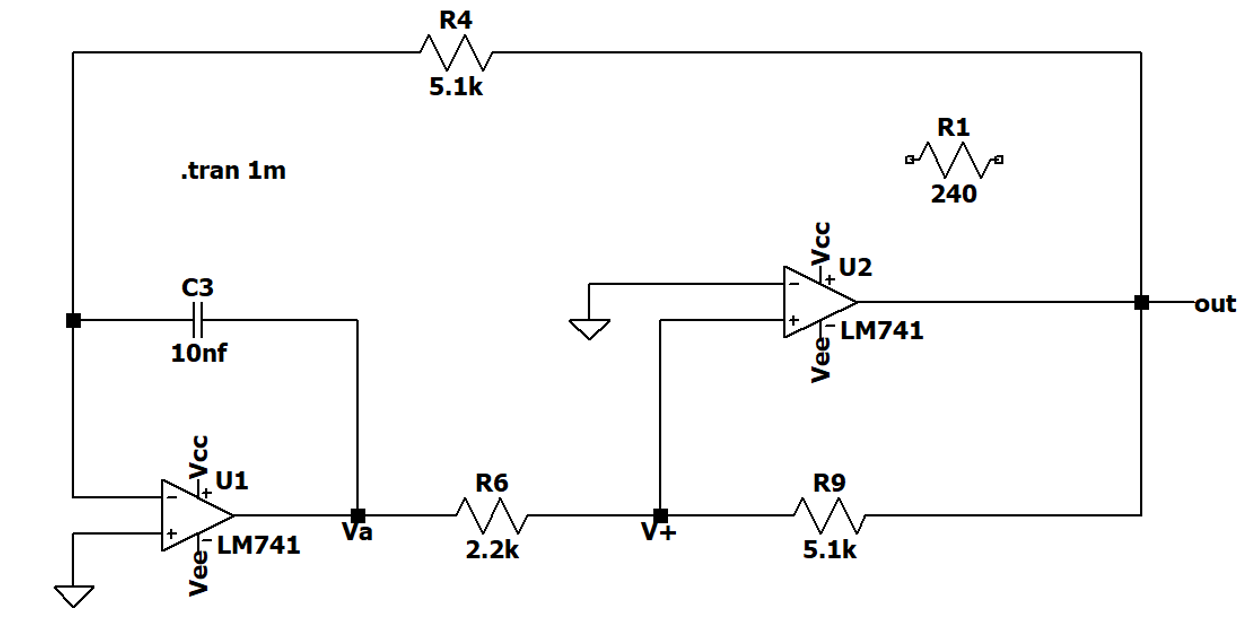
\includegraphics[width=10cm]{Circuitos/sim_gf_sindiodos.png}
                            \caption{Generador de funciones sin el regulador de voltaje}
                            \label{fig:gf_sindiodos}
                        \end{figure}
        
                        \begin{figure}[H]
                            \centering
                            \renewcommand{\figurename}{Gráfica}
                            \setcounter{figure}{11}
                            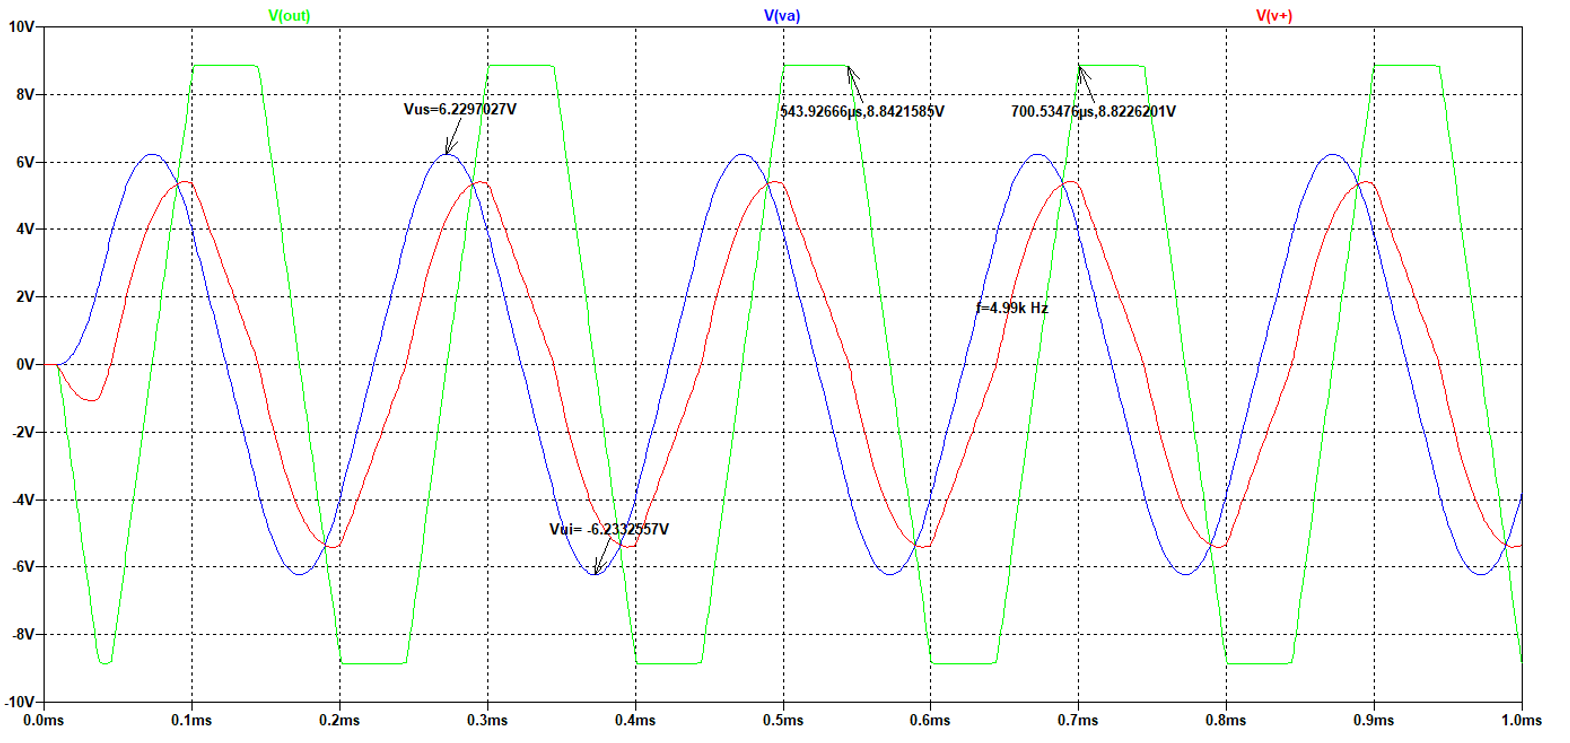
\includegraphics[width=10cm]{Imagenes/sim_gf_sindiodos.png}
                            \caption{Simulación de la señal de salida del circuito de la figura \ref{fig:gf} tanto del integrador como de la salida en general}
                            \label{fig:sim_gf_sindiodos}
                        \end{figure}

                    \item \textbf{Generador de funciones con regulador de funciones}

                         \begin{figure}[H]
                            \centering
                            \setcounter{figure}{19}
                            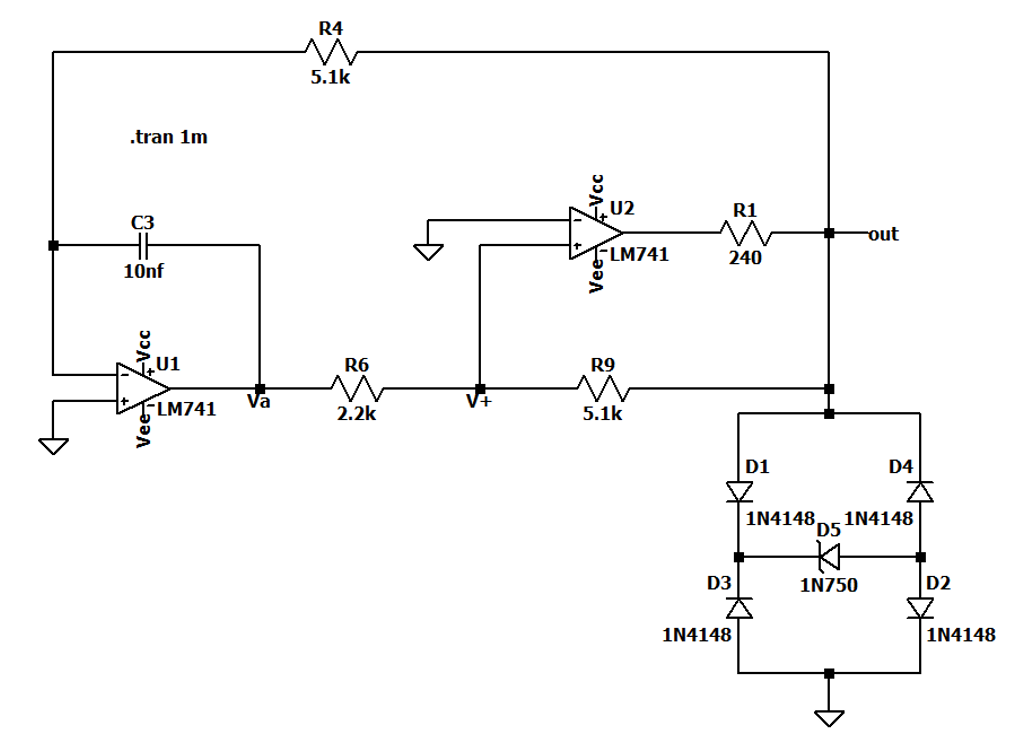
\includegraphics[width=10cm]{Circuitos/sim_cir_gf.png}
                            \caption{Generador de funciones}
                            \label{fig:sim_cir_gf}
                        \end{figure}
        
                        \begin{figure}[H]
                            \centering
                            \renewcommand{\figurename}{Gráfica}
                            \setcounter{figure}{12}  
                            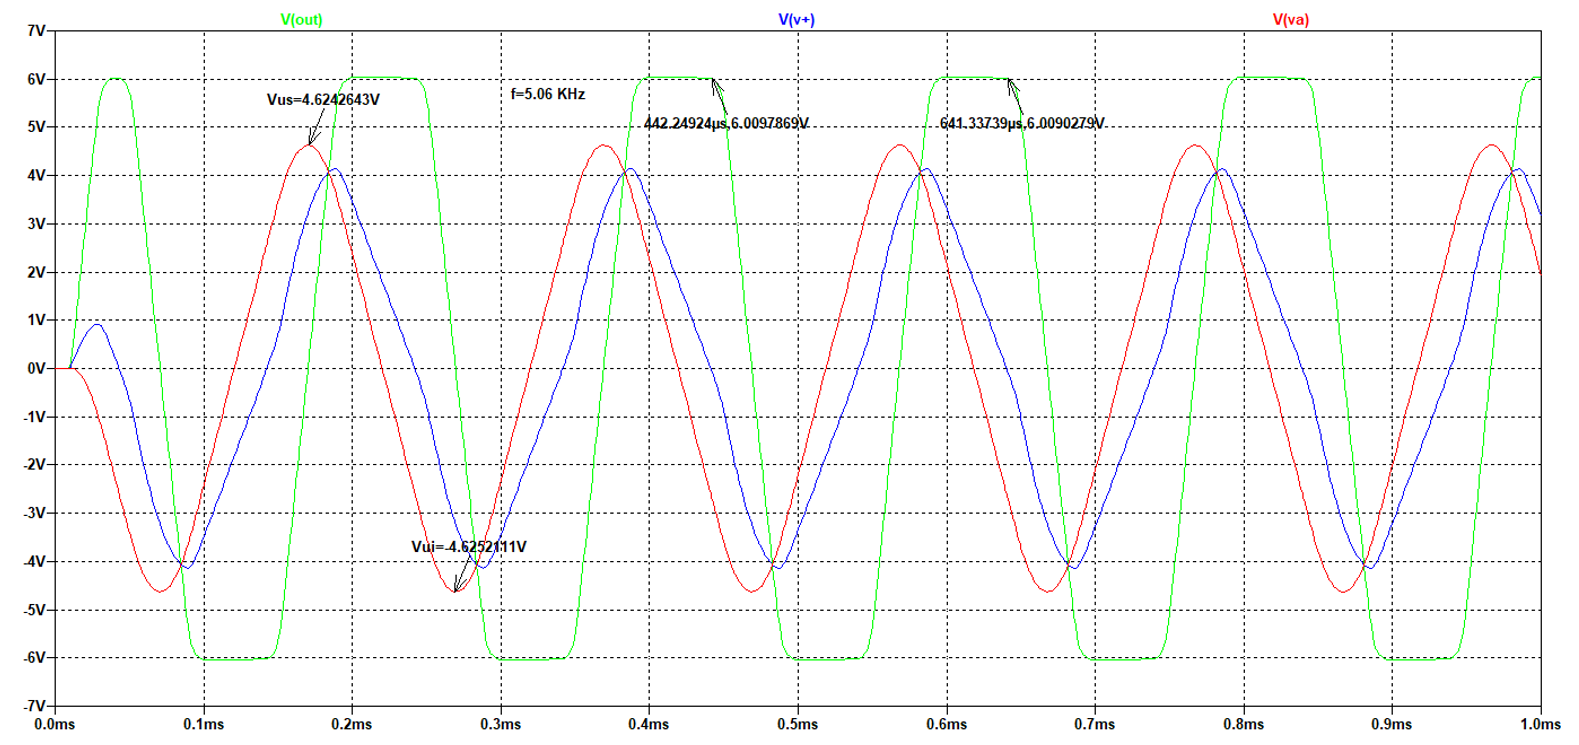
\includegraphics[width=10cm]{Imagenes/sim_gf.png}
                            \caption{Simulación de la señal de salida del circuito de la figura \ref{fig:gf} tanto del integrador como de la salida en general}
                            \label{fig:sim_gf}
                        \end{figure}

                \end{itemize}
                
            
        \end{enumerate}




    
\newpage

